 \documentclass[UTF8,a4paper,12pt]{ctexbook} 

 \usepackage{graphicx}%学习插入图
 \usepackage{verbatim}%学习注释多行
 \usepackage{booktabs}%表格
 \usepackage{geometry}%图片
 \usepackage{amsmath}
 \usepackage{amssymb}
 \usepackage{listings}%代码
 \usepackage{xcolor}  %颜色
 \usepackage{enumitem}%列表格式
 \usepackage{tcolorbox}
 \usepackage{algorithm}  %format of the algorithm
 \usepackage{algorithmic}%format of the algorithm
 \usepackage{multirow}   %multirow for format of table
 \usepackage{tabularx} 	%表格排版格式控制
 \usepackage{array}	%表格排版格式控制
 \usepackage{hyperref} %超链接 \url{URL}
\usepackage{dirtree}
 \CTEXsetup[format+={\flushleft}]{section}

 %%%% 段落首行缩进两个字 %%%%
 \makeatletter
 \let\@afterindentfalse\@afterindenttrue
 \@afterindenttrue
 \makeatother
 \setlength{\parindent}{2em}  %中文缩进两个汉字位
 
 
 %%%% 下面的命令重定义页面边距,使其符合中文刊物习惯 %%%%
 \addtolength{\topmargin}{-54pt}
 \setlength{\oddsidemargin}{0.63cm}  % 3.17cm - 1 inch
 \setlength{\evensidemargin}{\oddsidemargin}
 \setlength{\textwidth}{14.66cm}
 \setlength{\textheight}{24.00cm}    % 24.62
 
 %%%% 下面的命令设置行间距与段落间距 %%%%
 \linespread{1.4}
 % \setlength{\parskip}{1ex}
 \setlength{\parskip}{0.5\baselineskip}
 
 %%%% 下面的命令定义图表、算法、公式 %%%%
 \newcommand{\EQ}[1]{$\textbf{EQ:}#1\ $}
 \newcommand{\ALGORITHM}[1]{$\textbf{Algorithm:}#1\ $}
 \newcommand{\Figure}[1]{$\textbf{Figure }#1\ $}
 
 %%%% 下面命令改变图表下标题的前缀 %%%%% 如:图-1、Fig-1
 \renewcommand{\figurename}{Fig}
 
 \geometry{left=1.6cm,right=1.8cm,top=2cm,bottom=1.7cm} %设置文章宽度
 %%%% 设置图片目录
 \graphicspath{{figure/}}
 
 \pagestyle{plain} 		  %设置页面布局

 %代码效果定义
 \definecolor{mygreen}{rgb}{0,0.6,0}
 \definecolor{mygray}{rgb}{0.5,0.5,0.5}
 \definecolor{mymauve}{rgb}{0.58,0,0.82}
 \lstset{ %
 	backgroundcolor=\color{white},   % choose the background color
 	basicstyle=\footnotesize\ttfamily,      % size of fonts used for the code
 	%stringstyle=\color{codepurple},
 	%basicstyle=\footnotesize,
 	%breakatwhitespace=false,         
 	%breaklines=true,                 
 	%captionpos=b,                    
 	%keepspaces=true,                 
 	%numbers=left,                    
 	%numbersep=5pt,                  
 	%showspaces=false,                
 	%showstringspaces=false,
 	%showtabs=false,        
 	columns=fullflexible,
 	breaklines=true,                 % automatic line breaking only at whitespace
 	captionpos=b,                    % sets the caption-position to bottom
 	tabsize=4,
 	commentstyle=\color{mygreen},    % comment style
 	escapeinside={\%*}{*)},          % if you want to add LaTeX within your code
 	keywordstyle=\color{blue},       % keyword style
 	stringstyle=\color{mymauve}\ttfamily,     % string literal style
 	frame=single,
 	rulesepcolor=\color{red!20!green!20!blue!20},
 	% identifierstyle=\color{red},
 	language=c++,
 }
 \author{\kaishu 郑华}
 \title{\heiti 图形学理论 笔记}
 
\begin{document}          %正文排版开始
 	\maketitle
 	\tableofcontents
 		
\chapter{背景知识}
	\section{绪论}
		计算机图形学是利用计算机研究图形的表示、生成、处理、显示的学科。
		
		\subsection{应用与意义}
			\begin{itemize}
				\item 电影 :科幻大片的特效
				\item 游戏 :图形地理、人物控制
				\item 计算机仿真
				\item CAD/CAM :设计、制造
	 			\item 建筑
				\item 可视化(科学):化学结构、生物
			\end{itemize}	
	
		\subsection{研究内容}
			\begin{itemize}
				\item 图形硬件、图形标准、图形交互技术
				\item 光栅图形生成算法
				\item 曲线曲面造型、实体造型
				\item 真实感图形绘制、科学计算可视化、计算机动画、自然景物仿真
				\item 虚拟现实
			\end{itemize}
			
	\section{涉及概念}
		\paragraph{图形与图象}
			\subparagraph{图像}
				计算机内以位图(Bitmap)形式存在的灰度信息。
		
			\subparagraph{图形}
				含有几何属性、更强调场景的几何表示,是由场景的几何模型和景物的物理属性共同组成的。
				
				图形主要分为两种:
				\begin{itemize}[itemindent = 1em]
					\item 基于线条信息表示
					\item 明暗图(\textbf{Shading})
				\end{itemize}
		
		\paragraph{图形学与CAD}
		\paragraph{图形学与模式识别}
		\paragraph{图形学与视觉}

	\section{历史}
		\begin{itemize}
			\item 细分曲面
			\item 光栅化图形:区域填充、裁剪、消隐等基本图形概念(70年代)
			\begin{enumerate}
				\item 光反射模型 70年(真实感图形学)
				\item 漫反射模型+插值 71年(明暗处理)
				\item 简单光照模型 75年(Phong 模型)
				\item 光投射模型 80年,并给出光线跟踪算法范例(Whitted 模型)
				\item 辐射度方法 84年
			\end{enumerate}

		\end{itemize}
		
	\section{杂志与会议}
		\paragraph{会议}
		\begin{itemize}
			\item Siggraph 
			\item Eurograph
			\item Pacific Graphics
			\item Computer Graphics International.
		\end{itemize}
		
		\paragraph{杂志}
			\begin{itemize}
				\item ACM Transaction on Graphics
				\item IEEE Computer Graphics and Application
				\item IEEE Visualization and Computer Graphics
			\end{itemize}


	\section{真实感绘制及重要概念}
		目的是模拟真实物体的物理属性,包括物体的形状,光学性质,表面的纹理和粗燥程度,以及物体间的相对位置,遮挡关系等。
		
		\dirtree{%
			.1 图形学理论.
			.2 \textbf{光照模型}.
			.3 简单光照模型.
			.3 局部光照模型.
			.3 整体光照模型.
			.2 \textbf{绘制方法}.
			.3 光线追踪.
			.3 辐射度.
			.2 \textbf{加速算法}.
			.3 包围盒树、自适应八叉树等.
			.3 阴影算法、纹理合成.
		}


\chapter{数学基础}
	参考:\url{https://blog.csdn.net/wangdingqiaoit/article/details/51383052}
	\section{向量}
		\subsection{点积}
	
		\subsection{差积}
		
	
	\section{矩阵}
		
	\section{积分}
	
	\section{概率}

	\section{GLM库}
	
	
	
	
	
\chapter{渲染管线}
	在给定虚拟相机、三维物体、光源、照明模式,以及纹理等诸多条件的情况下,生成或绘制出一幅2维图像的过程。
		\begin{figure}[H]
			\centering
			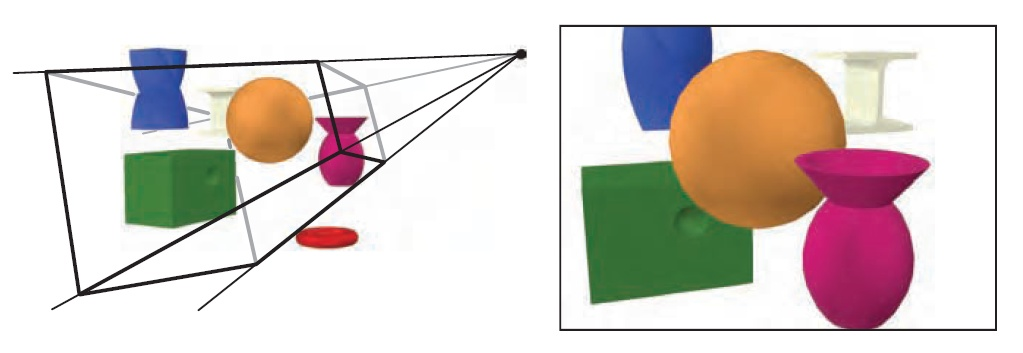
\includegraphics[scale=0.5]{Outline}
			\caption{渲染概述-三维到二维}
		\end{figure}
		
		而大体可以分为三部分:
		
		\begin{figure}[H]
			\centering
			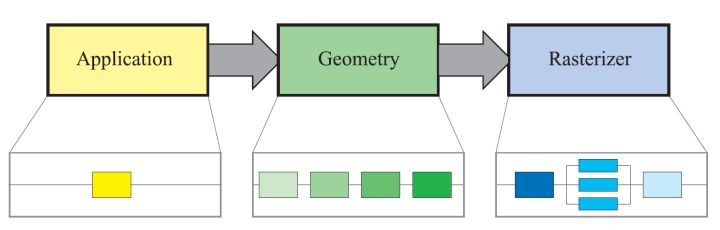
\includegraphics[scale=0.7]{Outline2}
			\caption{渲染结构}
		\end{figure}
		
	\section{应用阶段 - The Application Stage}
		应用程序阶段一般是图形渲染管线概念上的第一个阶段。应用程序阶段是通过软件方式来实现的阶段,开发者能够对该阶段发生的情况进行完全控制,可以通过改变实现方法来改变实际性能。其他阶段,他们全部或者部分建立在硬件基础上,因此要改变实现过程会非常困难。
		
		正因应用程序阶段是软件方式实现,因此不能像几何和光栅化阶段那样继续分为若干个子阶段。但为了提高性能,该阶段还是可以在几个并行处理器上同时执行。在CPU设计上,称这种形式为超标量体系(superscalar)结构,因为它可以在同一阶段同一时间做不同的几件事情。
		
		应用程序阶段通常实现的方法有\textbf{碰撞检测}、\textbf{加速算法}、\textbf{输入检测},\textbf{动画},\textbf{力反馈}以及\textbf{纹理动画},\textbf{变换仿真}、\textbf{几何变形},以及一些不在其他阶段执行的计算,如\textbf{层次视锥裁剪等加速算法}就可以在这里实现。
		
		应用程序阶段的主要任务:在应用程序阶段的末端,将需要在屏幕上(具体形式取决于具体输入设备)显示出来绘制的几何体(也就是绘制图元,rendering primitives,如点、线、矩形等)输入到绘制管线的下一个阶段。
		
		对于被渲染的每一帧,应用程序阶段将摄像机位置,光照和模型的图元输出到管线的下一个主要阶段——几何阶段。
		
	
	\section{几何阶段 - The Geometry Stage}
		负责大部分多边形操作和顶点操作。
			\begin{figure}[H]
				\centering
				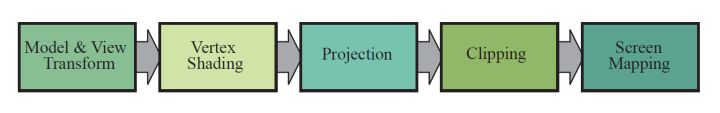
\includegraphics[scale=0.7]{Geometry}
				\caption{几何阶段演示}
			\end{figure}
		\subsection{模型视图变换阶段 - Model and View Transform} 
		
			模型变换的目的是将模型变换到适合渲染的空间当中,而视图变换的目的是\textbf{将摄像机位置放置于坐标原点},方便后续步骤的操作。
			
			在屏幕上的显示过程中,模型通常需要变换到若干不同的空间或坐标系中。模型变换的变换对象一般是模型的顶点和法线。物体的坐标称为模型坐标。世界空间是唯一的,所有的模型经过变换后都位于同一个空间中。
			
			不难理解,应该仅对相机(或者视点)可以看到的模型进行绘制。而相机在世界空间中有一个位置方向,用来放置和校准相机。
			
			为了便于投影和裁剪,必须对相机和所有的模型进行视点变换。变换的目的就是要把相机放在原点,然后进行视点校准,使其朝向Z轴负方向,y轴指向上方,x轴指向右边。在视点变换后,实际位置和方向就依赖于当前的API。我们称上述空间为\textbf{相机空间或者观察空间}。
		
				\begin{figure}[H]
					\centering
					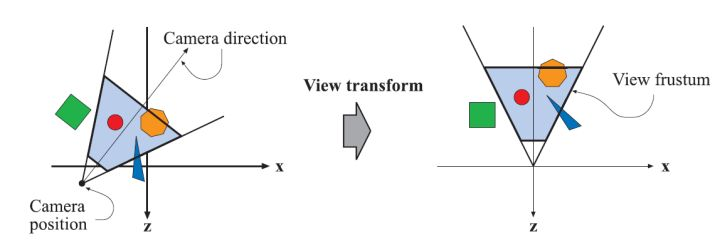
\includegraphics[scale=0.66]{ModelViewTransform}
					\caption{视图变换}
				\end{figure}
			
			在左图中,摄像机根据用户指定的位置进行放置和定位。在右图中,视点变换从原点沿着Z轴负方向对相机重新定位,这样可以使裁剪和投影操作更简单、更快速。可视范围是一个平截椎体,因此可以认为它是透视模式。	
			
			\subparagraph{总结}模型和视图变换阶段分为模型变换和视图变换。\textbf{模型变换}的目的是将模型变换到适合渲染的空间当中,而\textbf{视图变换}的目的是将摄像机放置于坐标原点,方便后续步骤的操作。
			
		\subsection{顶点着色阶段 - Vertex Shading} 
			顶点着色的目的在于\textbf{确定}模型上的\textbf{顶点处}材质的\textbf{光照效果}及\textbf{颜色}值。
			
			\color{blue}确定材质上的光照效果的这种操作被称为着色(shading),\color{black}着色过程涉及在对象上的各个点处计算\textbf{着色方程}(shading equation)。
			
			通常,这些计算中的一些在几何阶段期间在模型的顶点上执行(vertex shading),而其他计算可以在每像素光栅化(per-pixel rasterization)期间执行。\textbf{可以在每个顶点处存储各种材料数据},\textit{诸如点的位置,法线,颜色或计算着色方程所需的任何其它数字信息}。\color{red}\textbf{顶点着色的结果}(其可以是颜色,向量,纹理坐标或任何其他种类的阴着色数据)计算完成后,\textbf{会被发送到光栅化阶段以进行插值操作}。\color{black}
			
			通常,着色计算通常认为是在世界空间中进行的。在实践中,有时需要将相关实体(诸如相机和光源)转换到一些其它空间(诸如模型或观察空间)并在那里执行计算,也可以得到正确的结果。这是因为如果着色过程中所有的实体变换到了相同的空间,\textbf{着色计算中需要的诸如光源,相机和模型之间的相对关系是不会变的}。
			
		\subsection{投影阶段 - Projection} 
			就是将模型从三维空间投射到二维空间中的一个过程。
			
			在光照处理之后,渲染系统就开始进行投影操作,即将视体变换到一个对角顶点分别是(-1,-1,-1)和(1,1,1)单位立方体(unit cube)内,这个单位立方体通常也被称为规范立方体(Canonical View Volume,CVV)。
			目前,主要有两种投影方法,即:
			\begin{itemize}
				\item 正交投影:(orthographic projection,或称parallel projection)
				\item 透视投影:(perspective projection)。
			\end{itemize}
			
			\begin{figure}[H]
				\centering
				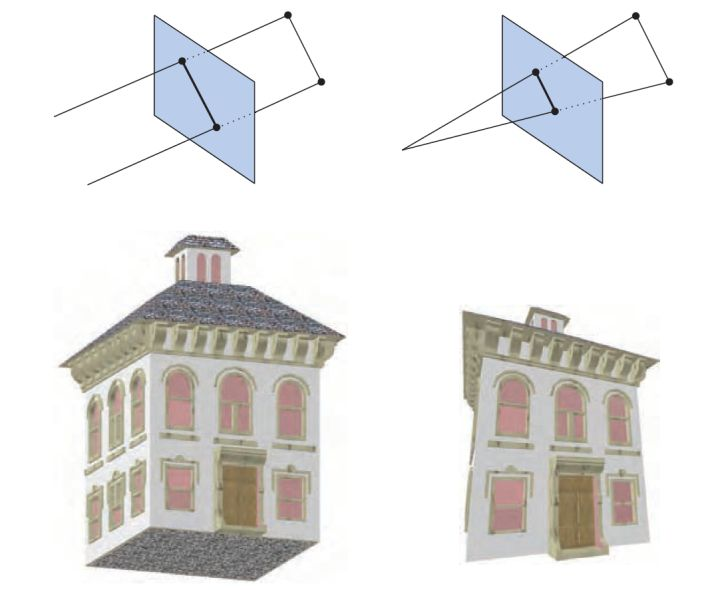
\includegraphics[scale=0.57]{project}
				\caption{投影演示}
			\end{figure}
			
			左边为正交投影,右边为透视投影。\textbf{正交投影}的可视体通常是一个矩形,正交投影可以把这个视体变换为单位立方体。正交投影的主要特性是平行线在变换之后彼此之间仍然保持平行,这种变换是平移与缩放的组合。\textbf{透视投影}比正交投影复杂一些。在这种投影中,越远离摄像机的物体,它在投影后看起来越小。更进一步来说,平行线将在地平线处会聚。透视投影的变换其实就是模拟人类感知物体的方式。
			
			正交投影和透视投影都可以通过4 x 4的矩阵来实现,在任何一种变换之后,都可以认为\textbf{模型位于归一化处理之后的设备坐标系中}。
			
			虽然这些矩阵变换是从一个可视体变换到另一个,但它们仍被称为投影,因为在完成显示后,\textbf{Z坐标将不会再保存于的得到的投影图片中}。通过这样的投影方法,\textbf{就将模型从三维空间投影到了二维的空间中}。
			
			\subparagraph{总结} 投影阶段就是将模型从三维空间投射到了二维的空间中的过程。
			
		\subsection{裁剪阶段 - Clipping} 
			就是对部分位于视体内部的图元进行裁剪操作。
			
			只有当图元完全或部分存在于视体(也就是上文的规范立方体,CVV)内部的时候,才需要将其发送到光栅化阶段,这个阶段可以把这些图元在屏幕上绘制出来。
			
			不难理解,一个图元相对视体内部的位置,分为三种情况:完全位于内部、完全位于外部、部分位于内部。所以就要分情况进行处理:
				\begin{itemize}
					\item 当图元完全位于视体内部,那么它可以直接进行下一个阶段。
					\item 当图元完全位于视体外部,不会进入下一个阶段,可直接丢弃,因为它们无需进行渲染。
					\item 当图元部分位于视体内部,则需要对那些部分位于视体内的图元进行裁剪处理。				
				\end{itemize}
			
			对部分位于视体内部的图元进行裁剪操作,这就是裁剪过程存在的意义。裁剪过程见下图。
				
				\begin{figure}[H]
					\centering
					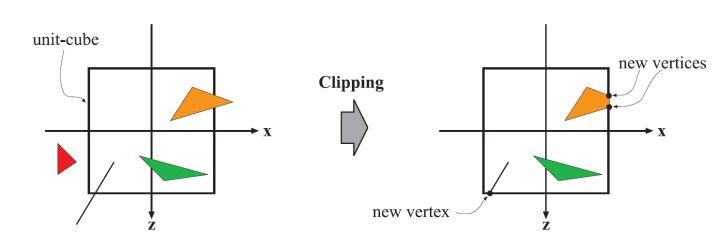
\includegraphics[scale=0.57]{clip}
					\caption{裁剪演示}
				\end{figure}
			
			投影变换后,\textbf{只对单位立方体内的图元}(\textit{相应的是视锥内可见图元})\textbf{继续进行处理},因此,\textbf{将单位立方体之外的图元剔除掉,保留单位立方体内部的图元},\textbf{同时沿着单位立方体将与单位立方体相交的图元裁剪掉},因此,就会产生新的图元,同时舍弃旧的图元。
			
		\subsection{屏幕映射阶段 - Screen Mapping} 
			就是将之前步骤得到的坐标映射到对应的屏幕坐标系上。
		
			只有在视体内部经过裁剪的图元,以及之前完全位于视体内部的图元,才可以进入到屏幕映射阶段。进入到这个阶段时,\textbf{坐标仍然是三维的}(\textbf{但显示状态在经过投影阶段后已经成了二维}),每个图元的x和y坐标变换到了屏幕坐标系中,屏幕坐标系连同z坐标一起称为窗口坐标系。
			
			假定在一个窗口里对场景进行绘制,窗口的最小坐标为(x1,y1),最大坐标为(x2,y2),其中x1<x2,y1<y2。屏幕映射首先进行平移,随后进行缩放,在映射过程中z坐标不受影响。新的x和y坐标称为屏幕坐标系,与z坐标一起(-1≦ z ≦ 1)进入光栅化阶段。如下图:
			
				\begin{figure}[H]
					\centering
					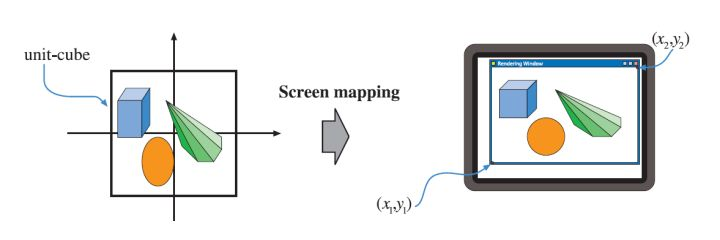
\includegraphics[scale=0.57]{scMap}
					\caption{屏幕映射演示}
				\end{figure}
	
			经过投影变换,图元全部位于单位立方体之内,而屏幕映射主要目的就是找到屏幕上对应的坐标
			
			屏幕映射阶段的一个常见困惑是整型和浮点型的点值如何与像素坐标(或纹理坐标)进行关联。可以使用Heckbert[书后参考文献第520篇]的策略,用一个转换公式进行解决。
			
			\subparagraph{总结}屏幕映射阶段的主要目的,就是将之前步骤得到的坐标映射到对应的屏幕坐标系上。
			
	\section{光栅化阶段 - The Rasterizer Stage}
		给定经过变换和投影之后的顶点,颜色以及纹理坐标,给每个像素正确配色,以便正确绘制整幅图像。
			\begin{figure}[H]
				\centering
				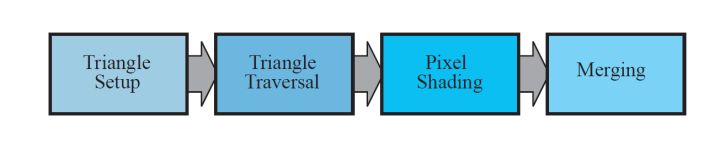
\includegraphics[scale=0.7]{Rasterization}
				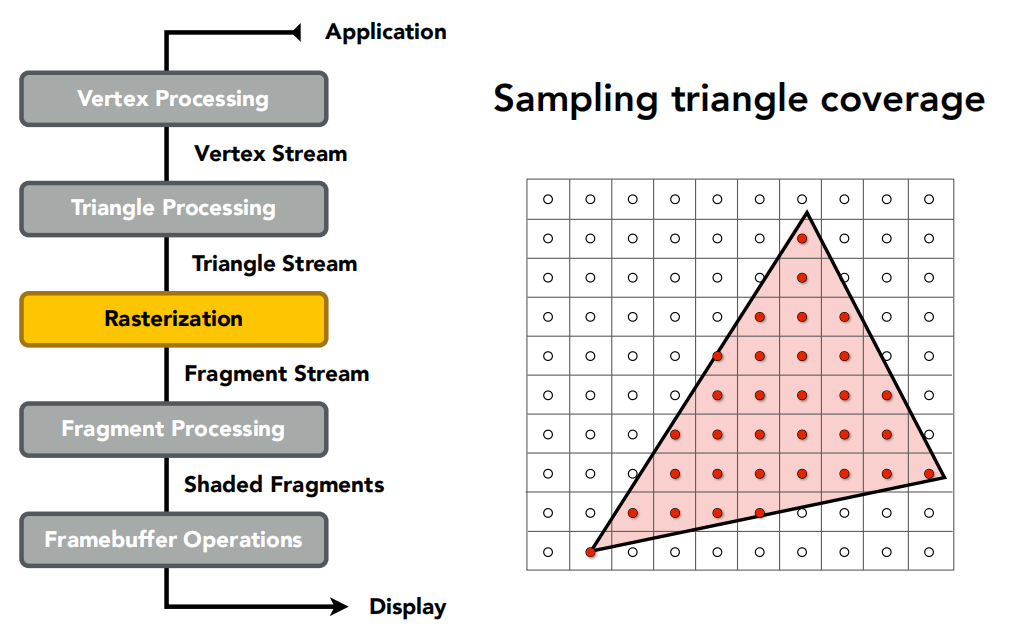
\includegraphics[width=\linewidth]{RasterizationPipeLine}
				\caption{光栅化演示}
			\end{figure}
			
			\subsection{三角形设定阶段 - Triangle Setup}
				三角形设定阶段主要用来计算三角形表面的差异和三角形表面的其他相关数据。
				
				该数据主要用于扫描转换(scan conversion),以及由几何阶段处理的各种着色数据的插值操作所用。 该过程在专门为其设计的硬件上执行。
				 
			\subsection{三角形遍历阶段 - Triangle Traversal}
				在三角形遍历阶段将进行\textbf{逐像素检查操作},\textbf{检查该像素处的像素中心是否由三角形覆盖},\textbf{而对于有三角形部分重合的像素,将在其重合部分生成片段(fragment)}。
				
				找到哪些采样点或像素在三角形中的过程通常叫三角形遍历(TriangleTraversal)或扫描转换(scan conversion)。\textbf{每个三角形片段的属性均由三个三角形顶点的数据插值而生成}。这些属性包括片段的深度,以及来自几何阶段的着色数据。

			\subsection{像素着色阶段 - Pixel Shading}
				所有逐像素的着色计算都在像素着色阶段进行,使用插值得来的着色数据作为输入,输出结果为一种或多种将被传送到下一阶段的颜色信息。纹理贴图操作就是在这阶段进行的。 其中主要有遮挡剔除的深度测试、提供基础色的纹理映射,以及明暗变化的光照渲染。
				
				\begin{figure}[H]
					\centering
					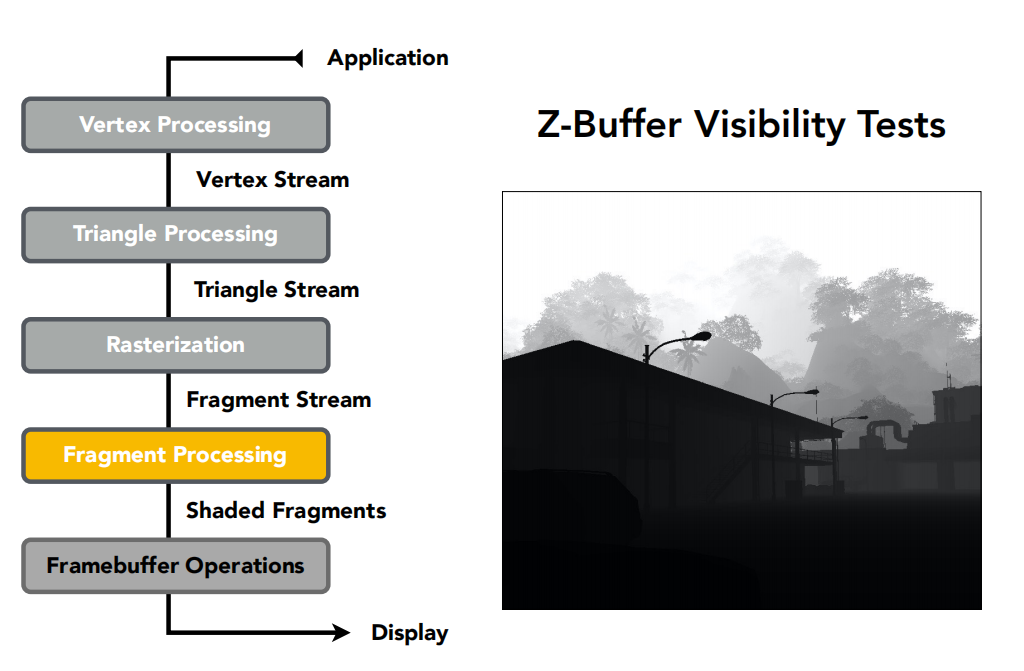
\includegraphics[scale=0.57]{Fragment-Test}
					\caption{片段着色器-测试}
				\end{figure}
				
				\begin{figure}[H]
					\centering
					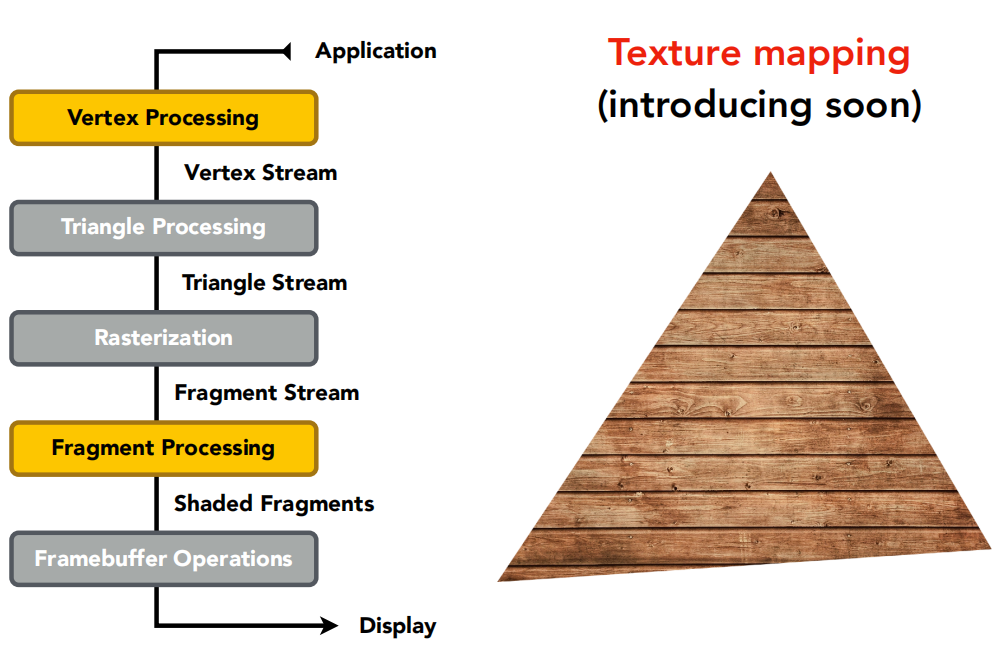
\includegraphics[scale=0.57]{Fragment-Texture}
					\caption{片段着色器-纹理映射}
				\end{figure}				
				
				\begin{figure}[H]
					\centering
					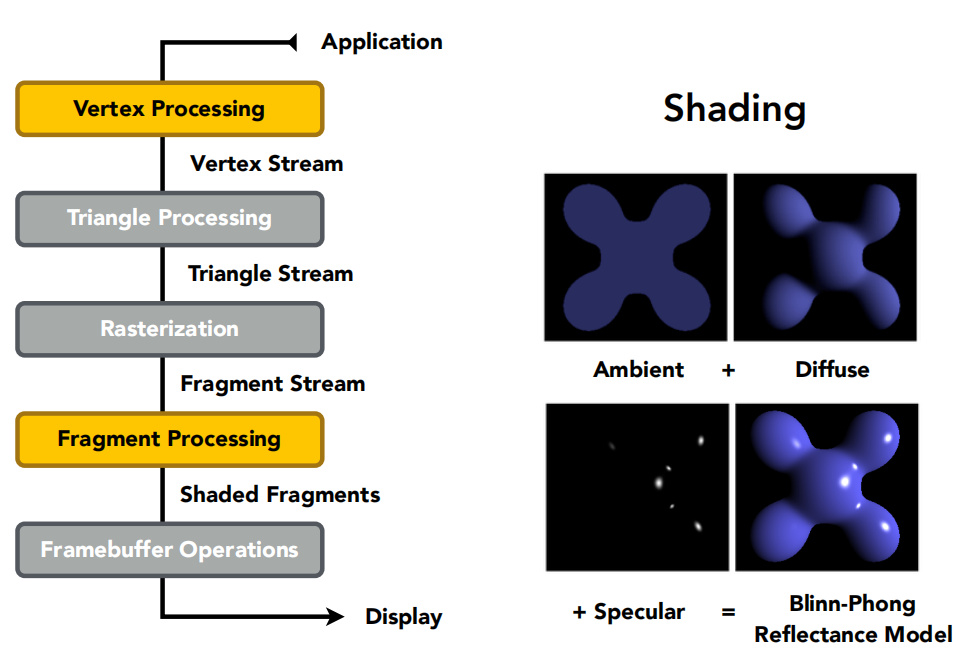
\includegraphics[scale=0.57]{Fragment-Light}
					\caption{片段着色器-光照着色}
				\end{figure}				
				
				像素着色阶段是在可编程GPU内执行的,在这一阶段有大量的技术可以使用,其中最常见,最重要的技术之一就是纹理贴图(Texturing)。纹理贴图在书的第六章会详细讲到。简单来说,纹理贴图就是将指定图片“贴”到指定物体上的过程。而指定的图片可以是一维,二维,或者三维的,其中,自然是二维图片最为常见。如下图所示:
					\begin{figure}[H]
						\centering
						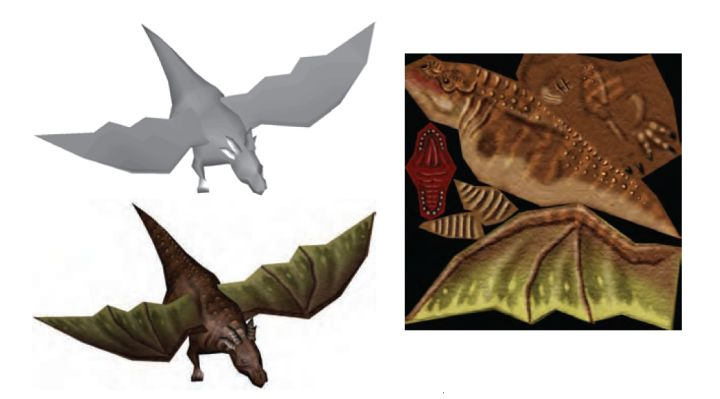
\includegraphics[scale=0.57]{PixShader}
						\caption{片段着色器演示}
					\end{figure}
				
				左上角为一没有纹理贴图的飞龙模型。左下角为一贴上图像纹理的飞龙。右图为所用的纹理贴图。
				
			\subsection{融合 - Merging}
				每个像素的信息都储存在\textbf{颜色缓冲器}中,而颜色缓冲器是一个颜色的矩阵列(每种颜色包含红、绿、蓝三个分量)。融合阶段的主要任务是合成当前储存于缓冲器中的由之前的像素着色阶段产生的片段颜色。不像其它着色阶段,通常运行该阶段的GPU子单元并非完全可编程的,但其高度可配置,可支持多种特效。
				
				此外,这个阶段还负责可见性问题的处理。这意味着当绘制完整场景的时候,颜色缓冲器中应该还包含从相机视点处可以观察到的场景图元。对于大多数图形硬件来说,这个过程是通过Z缓冲(也称\textbf{深度缓冲器})算法来实现的。Z缓冲算法非常简单,具有O(n)复杂度(n是需要绘制的像素数量),只要对每个图元计算出相应的像素z值,就可以使用这种方法,大概内容是:
				
				\textbf{Z缓冲器器}和颜色缓冲器形状大小一样,每个像素都存储着一个z值,这个z值是从相机到最近图元之间的距离。每次将一个图元绘制为相应像素时,需要计算像素位置处图元的z值,并与同一像素处的z缓冲器内容进行比较。如果新计算出的z值,远远小于z缓冲器中的z值,那么说明即将绘制的图元与相机的距离比原来距离相机最近的图元还要近。这样,像素的z值和颜色就由当前图元对应的值和颜色进行更新。反之,若计算出的z值远远大于z缓冲器中的z值,那么z缓冲器和颜色缓冲器中的值就无需改变。
														
				上面刚说到,颜色缓冲器用来存储颜色,z缓冲器用来存储每个像素的z值,还有其他缓冲器可以用来过滤和捕获片段信息。
				
				\begin{itemize}	
					\item 比如\textbf{alpha通道}(alpha channel)和\textbf{颜色缓冲器}\textit{联系在一起}可以存储一个与每个像素相关的不透明值。可选的alpha测试可在深度测试执行前在传入片段上运行。片段的alpha值与参考值作某些特定的测试(如等于,大于等),如果片断未能通过测试,它将不再进行进一步的处理。alpha测试经常用于不影响深度缓存的全透明片段(见6.6节)的处理。
									
					\item \textbf{模板缓冲器}(stencil buffer)是用于记录所呈现图元位置的离屏缓存。每个像素通常与占用8个位。图元可使用各种方法渲染到模板缓冲器中,而缓冲器中的内容可以控制颜色缓存和Z缓存的渲染。举个例子,假设在模版缓冲器中绘制出了一个实心圆形,那么可以使用一系列操作符来将后续的图元仅在圆形所出现的像素处绘制,类似一个mask的操作。模板缓冲器是制作特效的强大工具。而在管线末端的所有这些功能都叫做光栅操作(raster operations ,ROP)或混合操作(blend operations)。
									
					\item \textbf{帧缓冲器}(frame buffer)通常包含一个系统所具有的所有缓冲器,但有时也可以认为是颜色缓冲器和z缓冲器的组合。
									
					\item \textbf{累计缓冲器}(accumulation buffer),是1990年,Haeberli和Akeley提出的一种缓冲器,是对帧缓冲器的补充。这个缓冲器可以用一组操作符对图像进行累积。例如,为了产生运动模糊(motion blur.,可以对一系列物体运动的图像进行累积和平均。此外,其他的一些可产生的效果包括景深(e depth of field),反走样(antialiasing)和软阴影(soft shadows)等。
				\end{itemize}

				而当图元通过光栅化阶段之后,从相机视点处看到的东西就可以在荧幕上显示出来。为了避免观察者体验到对图元进行处理并发送到屏幕的过程,图形系统一般使用了双缓冲(double buffering)机制,这意味着屏幕绘制是在一个后置缓冲器(backbuffer)中以离屏的方式进行的。一旦屏幕已在后置缓冲器中绘制,后置缓冲器中的内容就不断与已经在屏幕上显示过的前置缓冲器中的内容进行交换。注意,只有当不影响显示的时候,才进行交换。
				
				\subparagraph{总结}融合阶段的主要任务是合成当前储存于缓冲器中的由之前的像素着色阶段产生的片段颜色。此外,融合阶段还负责可见性问题(Z缓冲相关)的处理。

	\section{可编程部分演示}
		\begin{figure}[H]
			\centering
			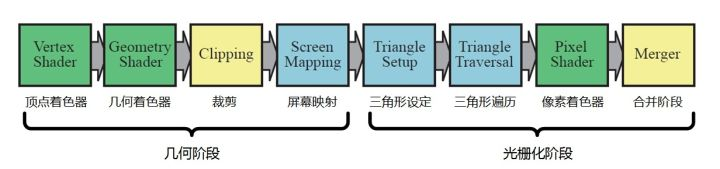
\includegraphics[scale=0.57]{ProgramAble}
			\caption{可编程阶段演示}
		\end{figure}	
		
		其中,\color{olive}绿色的阶段表示完全可编程的。\color{yellow}黄色表示可配置,但不可编程。\color{blue}蓝色的阶段完全固定。\color{black}
		
	\section{三大测试}
	
		在上述过程(片段着色器后)都完成后,将进入模版测试、深度测试、透明度测试。
	
		ref OPENGL 4.3 三大测试一章。


	\section{补充-重点}
		\subsection{混合}
		
		
		\subsection{背面剔除}
		
		
		\subsection{渲染队列}
			\url{https://blog.csdn.net/puppet_master/article/details/53900568}
		
	
	\section{前向渲染 Forward Rendering}
		Forward Rendering 是大多数渲染引擎使用的渲染技术。你给显卡提供几何对象,它将几何对象分解成顶点送入顶点着色器,然后把这些顶点数据插值后分别送入片元/像素着色器,然后在它们被送入屏幕前做最终的渲染处理(模板测试,混合等)。
	
		既传统的渲染顺序,也就是上文提到的顺序。
		
		\begin{figure}[H]
			\centering
			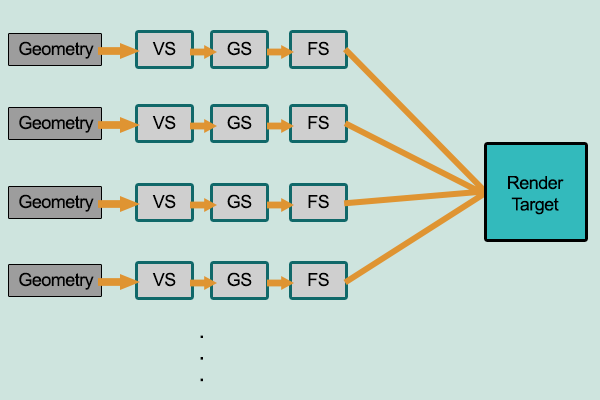
\includegraphics[width=.9\linewidth]{Forward}
			\caption{正向渲染:VS->FS->Render}
		\end{figure}
		

	\section{延迟渲染 Deferred Rendering}
		对前向渲染读下来,一定能发现一个问题,就是在3大测试前 在Fs中做了很多无用的计算,而这些计算又很耗时,因而为了解决这个问题,避免这些无用Fs(被测试丢弃的)的计算,提出来延迟渲染(Deferred Rendering)。
		
		延迟渲染,就是直到所有几何对象都已经通过渲染管线处理后,在最后才应用着色(通过光照来决定最终的像素颜色)并产生最终的图像。
		
		\begin{figure}[H]
			\centering
			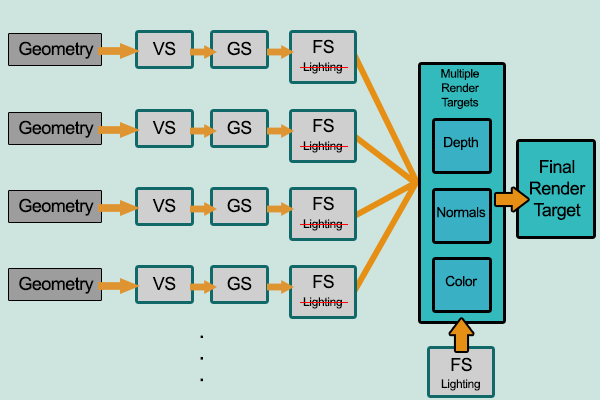
\includegraphics[width=.9\linewidth]{Defferred}
			\caption{延迟渲染}
		\end{figure}
		
		延迟照明是对延迟渲染的修改,通过在场景中使用\textbf{更多遍}来\textbf{减少G缓冲区}的大小。
		
		\subsection{改造原因分析}
			Lighting Performance(光照性能)。
			
			标准前向渲染(Forward Rendering)光照的性能消耗也是为什么要另辟蹊径选择其他渲染方式的主要原因。在标准前向渲染(Forward Rendering)管线流程中,每个灯光都会在每个顶点/或片元上执行光照计算,这也就是常说的逐顶点光照和逐片元/像素光照。
			
			如果你在场景中有100个几何对象,并且每个几何对象有1000个顶点,你大约就有100000多变形(非常粗略的计算)。显卡还能够很轻松的处理,但是当这些多边形被发送到片元着色器时, 昂贵的对灯光消耗会使性能急剧下降。开发者可以尝试放置光照计算到顶点着色器减少片元着色器对光照的计算。
			
			不管它是不是此像素上最顶层的片元,还是被遮挡的片元,昂贵的光照计算都会在每个多边形的每个可见片元上执行。如果屏幕的分辨率是1024x768,你有将近800000个像素需要被渲染。你能很轻易的就达到每帧百万级的片元操作。并且大多数的片元还会被剔除(深度测试阶段),那么对于此片元的光照就算就白费了。
			
			如果你要对这样一个达到百万级片元的场景的每一灯光进行渲染,那么你在每一帧将跃升的一个灯光数量x1000000个片元的操作上!
			
			计算前向渲染(Forward Rendering)复杂度的公式参见:复杂度公式:$O(num_{geometryFragments} * num_{lights})$。你能看到这里的复杂度是和几何对象数量和灯光数量直接相关的。
			
			片元是一个最终可能在屏幕上成为像素的一个”待转像素“,\textbf{如果在深度测试阶段不被剔除的话,它将在屏幕上成为屏幕的最终像素。}\textit{现在一些引擎通过其他的方式优化了光照计算,比如:剔除非常远的灯光,组合灯管或使用 Light maps(非常流行的,但是只能是静态的物体)}。如果你有大量的灯光需要动态光照的话,我们需要一个更好的解决方案。
			
			延迟渲染(Deferred Rendering)是一个减少光照着色对象数量有趣的方法。\textbf{尤其是对于总的片元对象来说,执行光照的片元数量直接由屏幕的分辨率决定}。
		
		\subsection{实现细节}
			每个几何对象被渲染,但是没有使用光照,使用多目标渲染(multiple render targets),绘制出多个屏幕空间大小的Buffer。深度,法线和颜色分别写入各自的buffers(图像)。然后,这些Buffers和每个灯光像的素颜色进行合成,最后生成最终的图像。
			
			\begin{figure}[H]
				\centering
				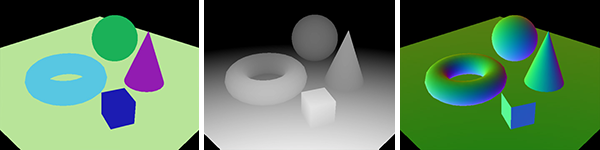
\includegraphics[width=\linewidth]{Defferred02}
				\caption{颜色、深度、正常缓冲区}
			\end{figure}
			
			\begin{figure}[H]
				\centering
				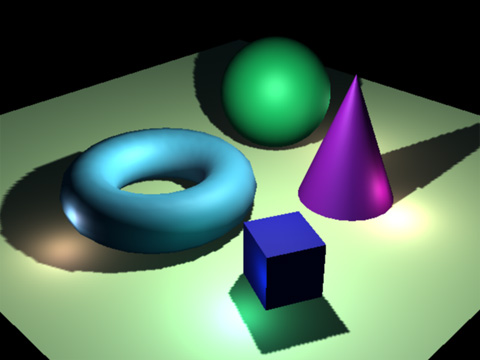
\includegraphics[width=\linewidth]{Defferred03}
				\caption{最终照明(阴影)使用三个缓冲区生成结果。}
			\end{figure}			
		
		
		\subsection{延迟渲染的缺点}
			• 这个处理需要显卡支持多目标渲染,老的显卡是不支持的,所有不能在上面工作,对于这个是没有变通的方案的,除非强制要求客服换显卡。
			
			• 它需要高带宽的显卡,你要发送大的Buffer数据,老大的显卡可能处理不了。对于这个也没有变通的方案的,除非强制要求客服换显卡。
			
			• 你不能使用透明对象。(除非你联合 使用deferred rendering 和Forward Rendering )。
			
			• 没有抗锯齿。
			
			• 仅有一个类型的材质被允许,除非你使用了被叫做Deferred Lighting的延迟渲染修改。
			
			• 阴影依赖于光照的数量,延迟渲染没有解决任何阴影的问题。	
			
		
			\textbf{如果}你没有大量的灯光或者你想能够在比较\textbf{老的显卡}上允许,你应该选择使用前向渲染(Forward Rendering)并且替换你的\textbf{灯光使用静态光照贴图}。
		
		
\chapter{变换 Transform MVP}
	见OpenGL\_4.5笔记


			
\chapter{纹理、贴图}
	\subsection{纹理概述}
		首先需要明确的是,纹理是用于给模型提供基础颜色的。而在三维世界的模型中的表面是可以通过变换形成一张2维的平面,如下所示。
	
		\begin{figure}[H]
			\centering
			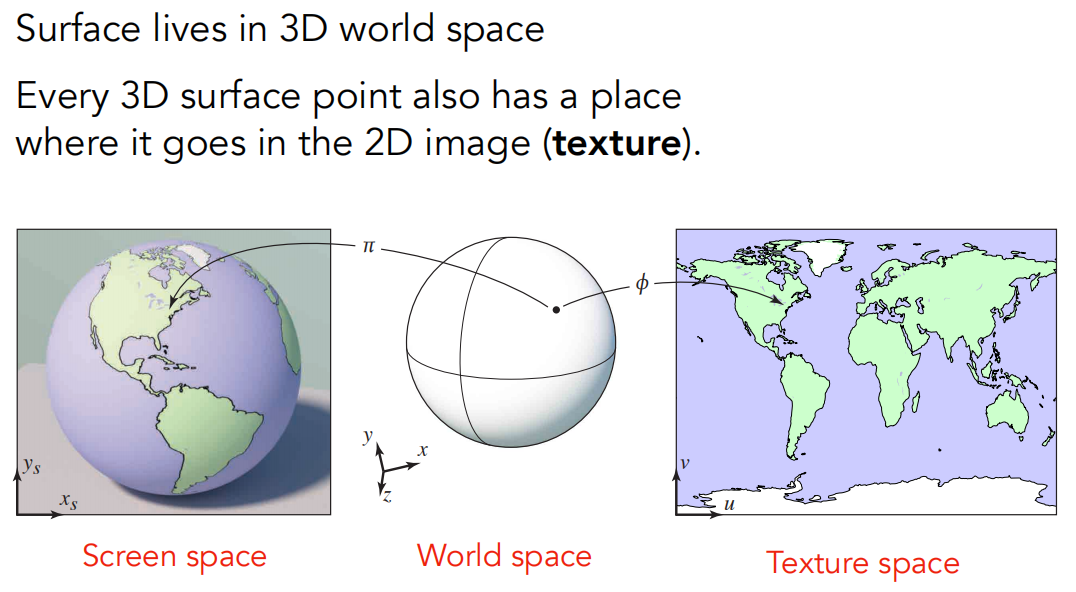
\includegraphics[width=\linewidth]{TextureMapping01}
			\caption{纹理映射原理示意}
		\end{figure}
		
		基于此原理,然后每个点或者叫像素,就可以唯一的与一个Texuure的像素对应,相应的,对于每一个三角形,都可以指定其中三个点的像素,然后在光栅化的过程中对三角形内进行像素插值。换句话说,纹理映射就是将Texture 中的三角形像素拷贝到模型中的三角形中,更进一步说,就是将模型中三角形的三个顶点的像素分别从Texture 上拷贝下来,然后在光栅化的时候会根据三个顶点的UV进行插值(\textit{三角形内的像素-UV插值})填充其余的。

		\begin{figure}[H]
			\centering
			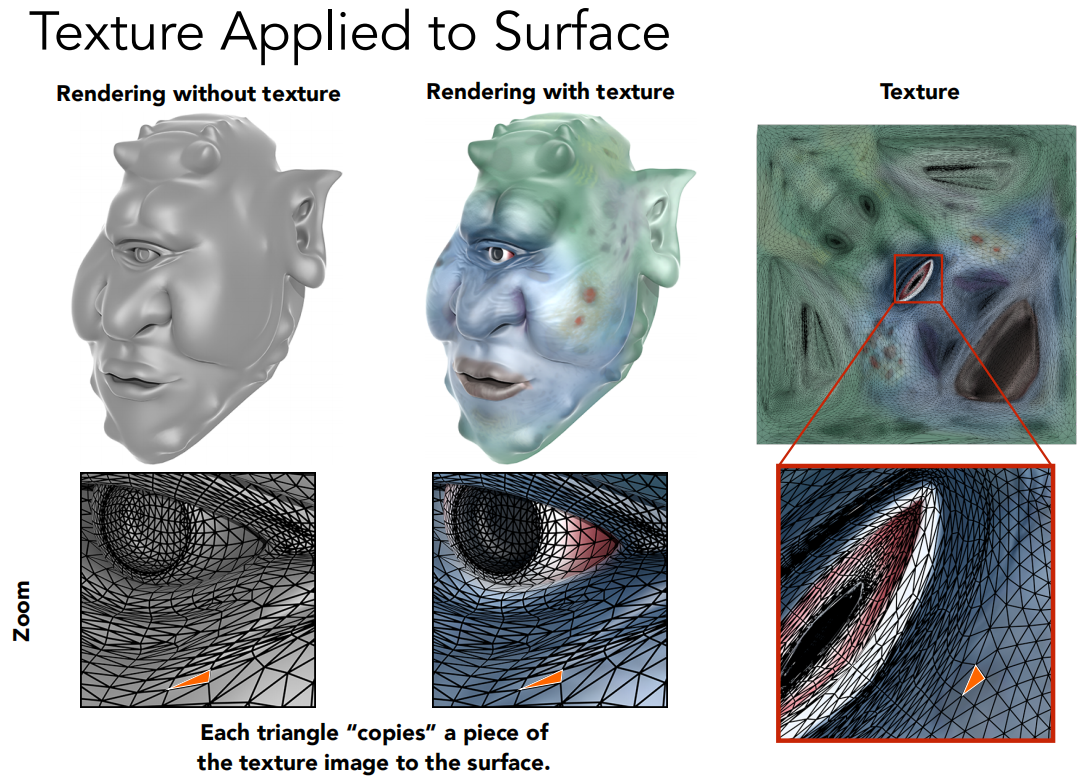
\includegraphics[width=\linewidth]{TextureMapping02}
			\caption{纹理映射到模型表面示意}
		\end{figure}

		\begin{figure}[H]
			\centering
			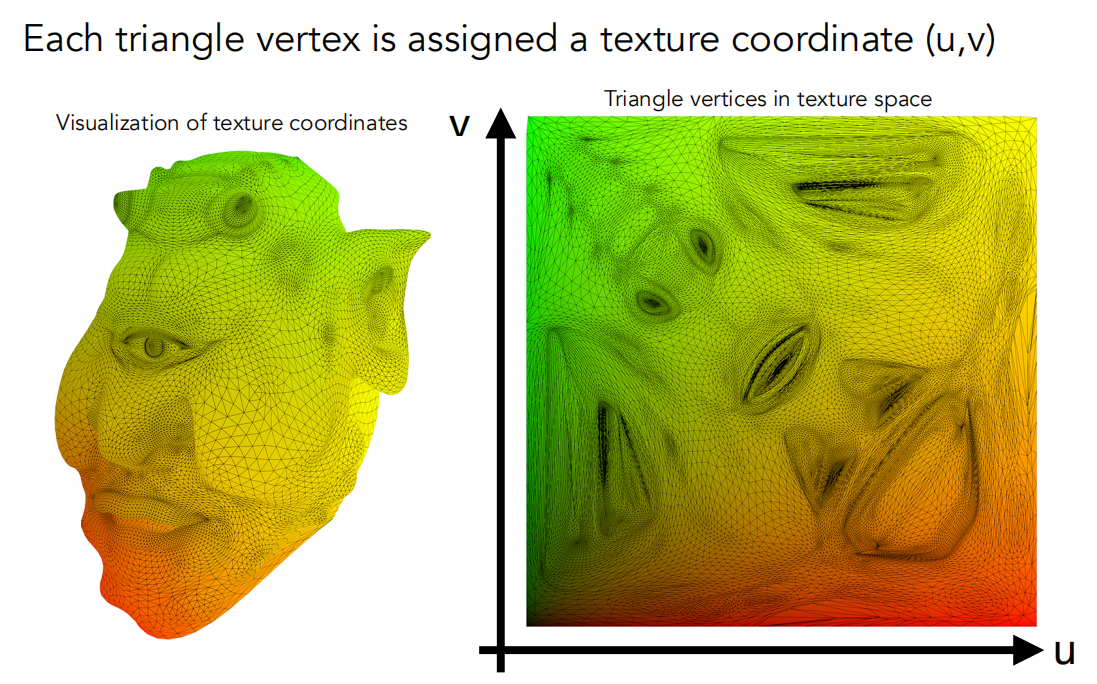
\includegraphics[width=\linewidth]{TextureMapping03}
			\caption{纹理与模型中的UV示意}
		\end{figure}
		
		最终的效果为:光栅化后的像素点根据(\textit{其三角形内重心坐标插值UV})确定其在纹理上的UV值,然后确定其颜色。
		\textbf{原来纹理的坐标都定义在三角形的顶点上,现在对于任何一个点,我们可以知道它在三角形的哪,就可以利用重心坐标做一个插值,算出这一个点的uv,然后在纹理上查询这个uv的值,也就是颜色值}。这个插值过程OpenGL或一些其他接口在光栅化的过程中会自动填充实现,在着色器中获取到的UV 直接使用即可。
		
		\textit{我们可以认为纹理定义的是漫反射的系数kd,这就等于把纹理贴在了物体上,并且这个物体还有blinn-phong带来的明暗变化。}
		
		\begin{figure}[H]
			\centering
			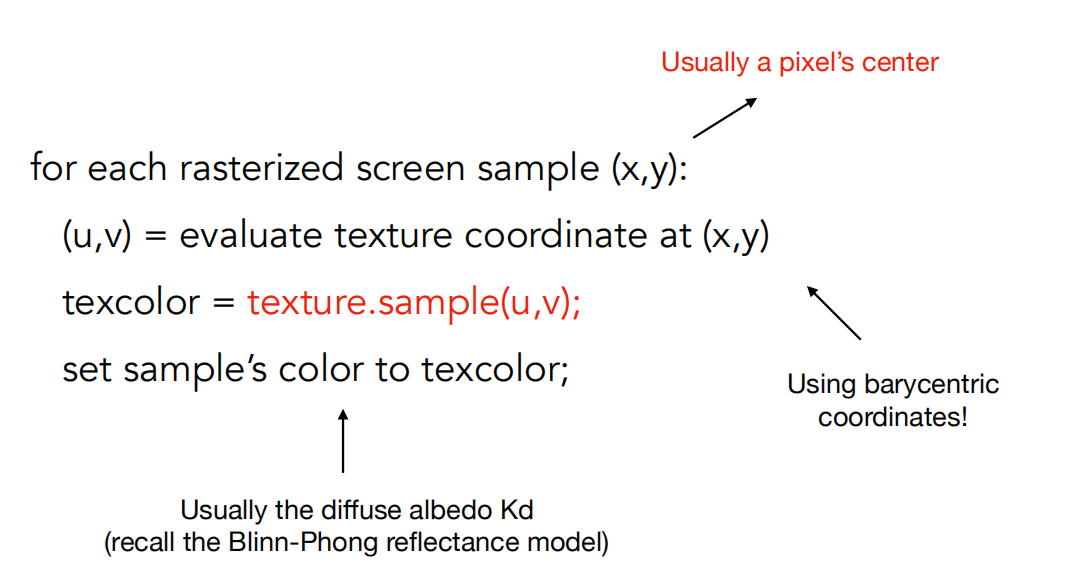
\includegraphics[width=\linewidth]{TextureMapping04}
			\caption{纹理映射流程:像素着色器中}
		\end{figure}

	

	\section{纹理管线}
		纹理(Texturing)是一种针对物体表面属性进行“建模”的高效技术。图像纹理中的像素通常被称为纹素(Texels),区别于屏幕上的像素。根据Kershaw的术语,\textit{通过将投影方程(projector function)运用于空间中的点 ,从而得到一组称为参数空间值(parameter-spacevalues)的关于纹理的数值}。这个过程就称为贴图(Mapping,也称映射 ),也就是\textbf{纹理贴图}(Texture Mapping,也称纹理映射 )这个词的由来。
		
		纹理贴图可以用一个通用的纹理管线来进行描述。纹理贴图过程的\textbf{初始点}是空间中的一个位置。这个位置\textbf{可以基于世界空间},但是\textbf{更常见的是基于模型空间}。因为若此位置是基于模型空间的,当模型移动时,其纹理才会随之移动。
		
		如下图为一个纹理管线(The Texturing Pipeline),也就是单个纹理应用纹理贴图的详细过程,而此管线有点复杂的原因是每一步均为用户提供了有效的控制。
			\begin{figure}[H]
				\centering
				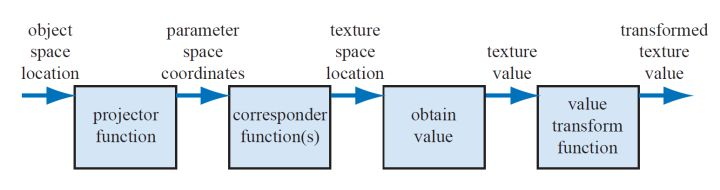
\includegraphics[scale=0.67]{TexturePipeline}
				\caption{单个纹理的通用纹理管线}
			\end{figure}
			
		下面是对上图中描述的纹理管线的分步概述:
			\begin{enumerate}[itemindent = 2em]
				\item 通过将投影方程(projector function)运用于空间中的点 ,从而得到一组称为参数空间值(parameter-space values)的\textbf{关于纹理的数值}。
				\item 在使用这些新值访问纹理之前,可以使用一个或者多个映射函数(corresponder function)将\textbf{参数空间值}(parameter-space values )转换到\textbf{纹理空间}。
				\item 使用这些纹理空间值(texture-space locations)\textbf{从纹理中获取相应的值}(obtain value)。例如,可以使用图像纹理的数组索引来检索像素值。
				\item 再使用值变换函数(value transform function)对检索结果进行值变换,最后使用得到的新值来改变表面属性,如材质或者着色法线等等。
			\end{enumerate}

		而如下这个例子应该对理解纹理管线有所帮助。下例将描述出使用纹理管线,一个多边形在给定一张砖块纹理时在其表面上生成样本时(如下图)发生了哪些过程。
			\begin{figure}[H]
				\centering
				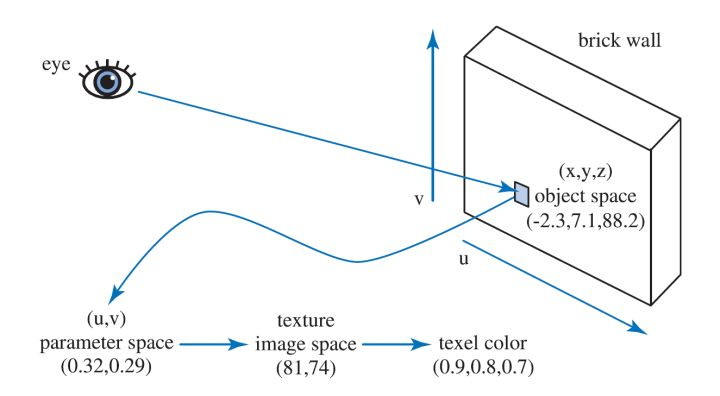
\includegraphics[scale=0.67]{TexturePipeline2}
				\caption{一个砖墙的纹理管线过程}
			\end{figure}
		
		在具体的参考帧画面中找到\textbf{物体空间中的位置(x,y,z)},如图中点(-2.3,7.1,88.2),然后\textbf{对该位置运用投影函数}。\color{blue}\textbf{这个投影函数通常将向量(x,y,z)转换为一个二元向量(u,v)}\color{black}。在此示例中使用的投影函数是一个正交投影,类似一个投影仪,将具有光泽的砖墙图像投影到多边形表面上。再考虑砖墙这边,其实这个投影过程就是将砖墙平面上的点变换为值域为0到1之间的一对(u,v)值,如图,(0.32,0.29)就是这个我们通过投影函数得到的uv值。\textbf{而我们图像(纹理)的分辨率是256 x 256,所以,将256分别乘以(0.32,0.29),去掉小数点,得到纹理坐标(81, 74)。}通过这个纹理坐标,可以\textbf{在纹理贴图上查找到坐标对应的颜色值},所以,我们接着找到砖块图像上像素位置为(81,74)处的点,得到颜色(0.9,0.8,0.7)。而由于原始砖墙的颜色太暗,因此可以使用一个值变换函数,给每个向量乘以1.1,就可以得到我们纹理管线过程的结果——颜色值(0.99,0.88,0.77)。
		
		随后,我们就可以将此值用于着色方程,作为物体的漫反射颜色值,替换掉之前的漫反射颜色。
		
		下面是纹理管线中主要的两个组成,投影函数(The Projector Function)和映射函数(The Corresponder Function)。
			
	\section{投影函数}
		作为\textbf{纹理管线的第一步},投影函数的功能就是\textbf{将空间中的三维点转化为纹理坐标},也就是\textbf{获取表面的位置并将其投影到参数空间中}。
		
		在常规情况下,投影函数通常在美术建模阶段使用,并将投影结果存储于顶点数据中。也就是说,在软件开发过程中,我们一般不会去用投影函数去计算得到投影结果,\textbf{而是直接使用在美术建模过程中,已经存储在模型顶点数据中的投影结果}。
		
	\section{映射函数}
		映射函数(The Corresponder Function)的作用是将参数空间坐标(parameter-space coordinates)转换为纹理空间位置(texture space locations)。
		
		我们知道图像会出现在物体表面的(u,v)位置上,且uv值的正常范围在[0,1)范围内。超出这个值域的纹理,其显示方式便可以由映射函数(The Corresponder Function)来决定。
		
		在OpenGL中,这类映射函数称为“封装模式(Warapping Mode)”,在Direct3D中,这类函数叫做“寻址模式(Texture Addressing Mode)”。最常见的映射函数有以下几种:
			
			\begin{figure}[H]
				\centering
				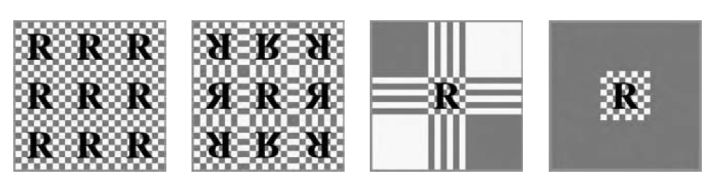
\includegraphics[scale=0.57]{Mapping}
				\caption{映射方式}
			\end{figure}
			
			\begin{itemize}
				\item \textbf{重复寻址模式},\verb|wrap| (DirectX), \verb|repeat| (OpenGL)。图像在表面上重复出现。
				\item \textbf{镜像寻址模式},\verb|mirror|。图像在物体表面上不断重复,但每次重复时对图像进行镜像或者反转。
				\item \textbf{夹取寻址模式},\verb|clamp| (DirectX) ,clamp to edge (OpenGL)。夹取纹理寻址模式将纹理坐标夹取在[0.0,1.0]之间,也就是说,在[0.0,1.0]之间就是把纹理复制一遍,然后对于[0.0,1.0]之外的内容,将边缘的内容沿着u轴和v轴进行延伸。
				\item \textbf{边框颜色寻址模式},\verb|border| (DirectX) ,clamp to border (OpenGL)。边框颜色寻址模式就是在[0.0,1.0]之间绘制纹理,然后[0.0,1.0]之外的内容就用边框颜色填充。		
			\end{itemize}

		另外,每个纹理轴可以使用不同的映射函数。例如在u轴使用重复寻址模式,在v轴使用夹取寻址模式。
		
	\section{体纹理}
	
	\section{立方体贴图}
		立方体纹理(cube texture)或立方体贴图(cube map)是一种特殊的纹理技术,它用6幅二维纹理图像构成一个以原点为中心的纹理立方体,这每个2D纹理是一个立方体(cube)的一个面。对于每个片段,纹理坐标(s, t, r)被当作方向向量看待,每个纹素(texel)都表示从原点所看到的纹理立方体上的图像。
		
			\begin{figure}[H]
				\centering
				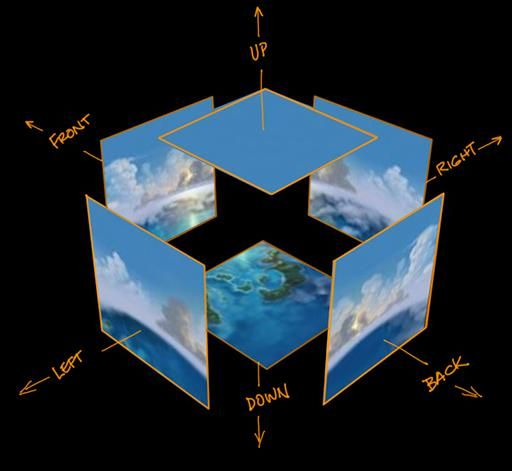
\includegraphics[scale=0.57]{cubeMap}
				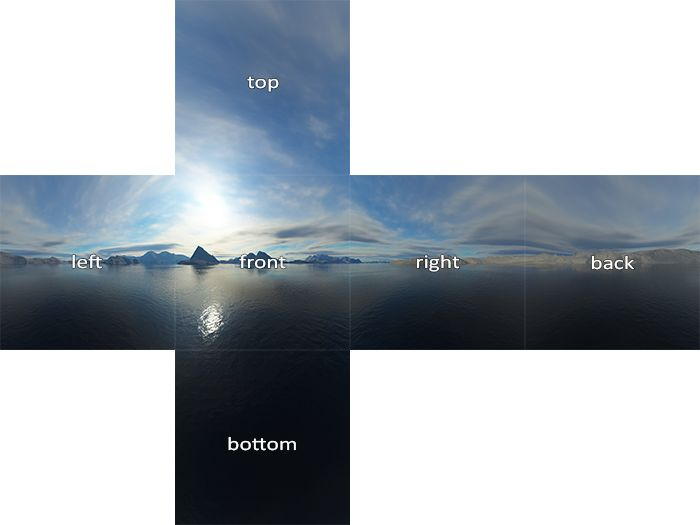
\includegraphics[scale=0.57]{cubeMap1}
				\caption{立方体贴图}
			\end{figure}
		
		可以使用三分量纹理坐标向量来访问立方体贴图中的数据,该矢量指定了从立方体中心向外指向的光线的方向。选择具有最大绝对值的纹理坐标对应的相应的面。(例如:对于给定的矢量(−3.2, 5.1, −8.4),就选择-Z面),而对剩下的两个坐标除以最大绝对值坐标的绝对值,即8.4。 那么就将剩下的两个坐标的范围转换到了-1到1,然后重映射到[0,1]范围,以方便纹理坐标的计算。例如,坐标(-3.2,5.1)映射到((-3.2 / 8.4 + 1)/ 2,(5.1/ 8.4 + 1)/ 2)≈(0.31,0.80)。
		
		立方体贴图支持\textbf{双线性滤波}以及\textbf{mip mapping},但问题可以可能会在贴图接缝处出现。有一些处理立方体贴图专业的工具在滤波时考虑到了可能的各种因素,如ATI公司的CubeMapGen,采用来自其他面的相邻样本创建\textbf{mipmap链},并考虑每个纹素的角度范围,可以得到比较不错的效果。
				
	\section{纹理缓存}
	
	\section{纹理压缩}
	
	\section{程序贴图纹理}
	
	\section{凹凸贴图}
		凹凸贴图(Bump Mapping)思想最早是由图形学届大牛中的大牛Jim Blinn提出,后来的Normal Mapping,Parallax Mapping,Parallax Occulision Mapping,Relief Mapping等等,均是基于同样的思想,只是考虑得越来越全面,效果也越来越逼真。
		
		\begin{figure}[H]
			\centering
			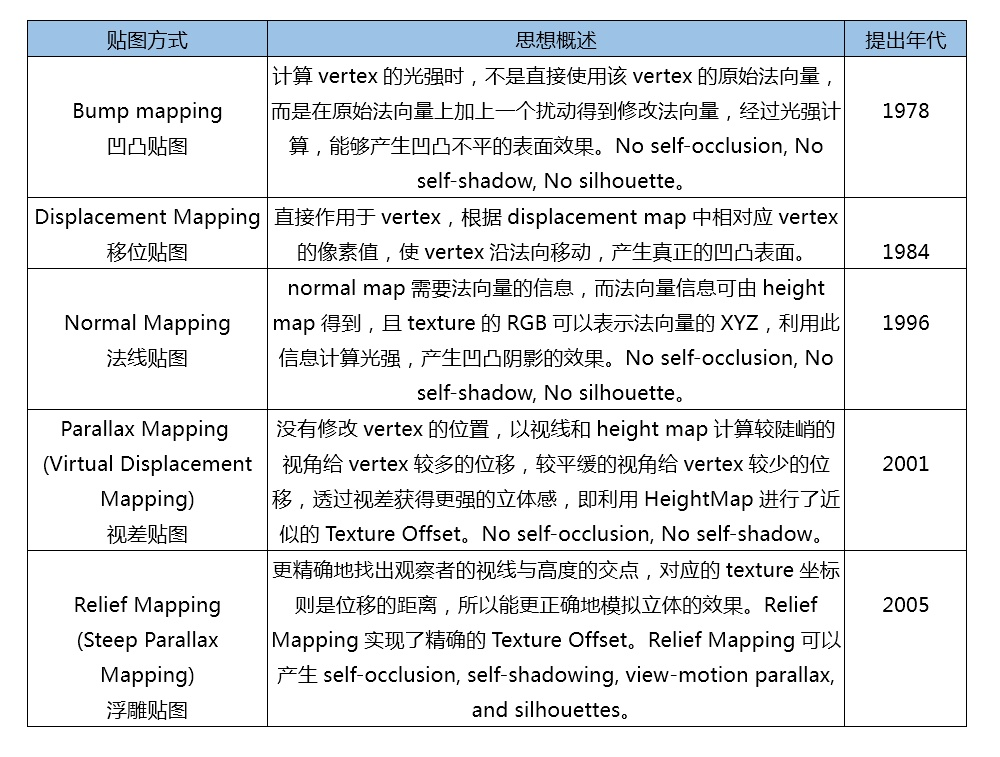
\includegraphics[scale=0.53]{normMap}
			\caption{凹凸贴图对比}
		\end{figure}
		
		凹凸贴图是指计算机图形学中在三维环境中\textbf{通过纹理方法}来产生表面凹凸不平的视觉效果。它主要的\textbf{原理是}\textit{通过改变表面光照方程的法线,而不是表面的几何法线,或对每个待渲染的像素在计算照明之前都要加上一个从高度图中找到的扰动},来模拟凹凸不平的视觉特征,如褶皱、波浪等等。	
		
			\paragraph{高度图或灰度图}
				一张二维纹理有两个维度 $u$ 和 $v$,但其实,高度($h$)可以算第三个维度。有了高度,一张二维纹理就可以想象成一个三维的物体了。
					\begin{figure}[H]
						\centering
						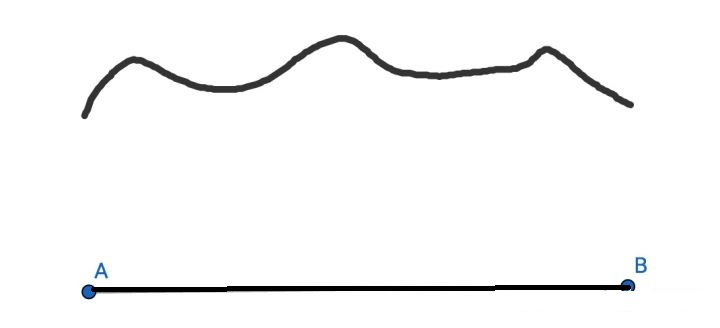
\includegraphics[scale=0.54]{norMap}
						\caption{UV例子}
					\end{figure}
				
				先来考虑只有 $u$ 方向的情况,如图所示, $A$ 和 $B$ 是纹理中的两个点, $uv$ 坐标分别是 (0, 0) 和 (1, 0),上方黑线表示点对应的高度,那么显然,只要求出 $u$ 方向上的高度函数在某一点的切线,就能求出垂直于他的法线了。同理, $v$ 方向也是如此。也就是说,如果有纹理的高度信息,那么就能计算出纹理中每一个像素的法线了。
				
				所以计算法线需要一张高度图,它表示纹理中每一个点对应的高度。
				
				但其实并不需要求出每个纹理像素上 $uv$ 方向各自的法线,只需要求出 $uv$ 方向上高度函数的切线,再做一个叉积,即可计算出对应的法线了。
				
				如果没有高度图,也可以用灰度图代替,灰度图就是把 $rgb$ 三个颜色分量做一个加权平均,有很多种算法提取灰度值,这里用一个比较常用的基于人眼感知的灰度值提取公式。
				
				$$color.r * 0.2126 + color.g * 0.7152 + color.b * 0.0722$$
				
				这个公式是由人眼对不同颜色敏感度不同得来的,这里无需过多计较,直接把提取出来的灰度值作为高度值即可。
				
						
		\subsection{移位贴图}
			Displacement Mapping,移位贴图,也有人称为置换贴图,或称高度纹理贴图(Heightfield Texturing)。这种方法类似于法线贴图,移位贴图的每一个纹素中存储了一个向量,这个向量代表了对应顶点的位移。注意,此处的纹素并不是与像素一一对应,而是与顶点一一对应,因此,纹理的纹素个数与网格的顶点个数是相等的。在VS阶段,获取每个顶点对应的纹素中的位移向量,施加到局部坐标系下的顶点上,然后进行世界视点投影变换即可。
		
		
		\subsection{法线贴图}
			ref:\url{https://zhuanlan.zhihu.com/p/102131805}
		
			法线贴图(Normal mapping)\textit{是凸凹贴图(Bump mapping)技术的一种应用},法线贴图有时也称为“\textit{Dot3(仿立体)凸凹纹理贴图}”。
			
			每个fragment使用了自己的法线,我们就可以让光照相信一个表面由很多微小的(垂直于法线向量的)平面所组成,物体表面的细节将会得到极大提升。\textit{这种每个fragment使用各自的法线,替代一个面上所有fragment使用同一个法线的技术叫做法线贴图(normal mapping)}。
			
			只需要改变每个fragment的法线向量,并不需要改变所有光照公式。\textbf{现在是为每个fragment传递一个法线,不再使用插值表面法线}。
			
			与凸凹纹理贴图(\textit{通常是在现有的模型法线添加扰动})不同,法线贴图要完全更新法线。与凸凹贴图类似的是,它也是用来在不增加多边形的情况下在浓淡效果中添加细节。但是\textbf{凸凹贴图}通常根据一个\textit{单独的灰度图像通道}进行计算,而\textbf{法线贴图}的数据源图像通常是从\textit{更加细致版本的物体得到的多通道图像},即红、绿、蓝通道都是作为一个单独的颜色对待。
		
			简单来说,Normal Map直接将正确的Normal值保存到一张纹理中去,那么在使用的时候直接从贴图中取即可。
			
			\begin{figure}[H]
				\centering
				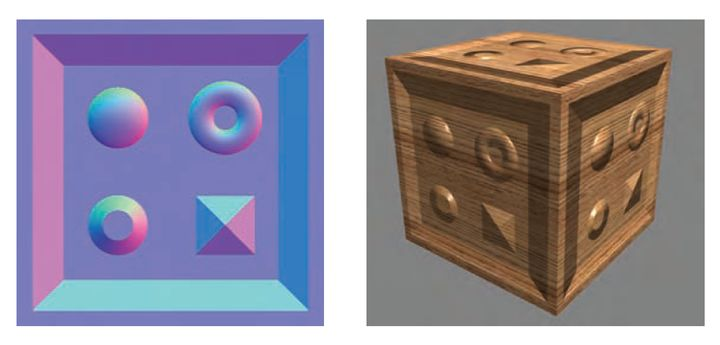
\includegraphics[width=\linewidth]{normalMap}
				\caption{法线贴图纹理:使用法线贴图生成的图像}
			\end{figure}
			
			基于法线贴图的凹凸映射,\textbf{每个颜色通道实际上是表面法线坐标。红色通道是x偏差; 红色越多,正常点越多。 绿色是y偏差,蓝色是z}。
			
			\paragraph{计算方法}
				ref:\url{https://learnopengl-cn.github.io/05%20Advanced%20Lighting/04%20Normal%20Mapping/}
				
				\subparagraph{法线纹理采样使用}
					为使法线贴图工作,我们需要为每个fragment提供一个法线。像diffuse贴图和specular贴图一样,我们可以使用一个2D纹理来储存法线数据。2D纹理不仅可以储存颜色和光照数据,还可以储存法线向量。这样我们可以从2D纹理中采样得到特定纹理的法线向量。
					
					由于纹理存储的值范围在[0,1], 而法线则是[-1,1], 因而需要一定变换使两个的范围一致。
					\begin{lstlisting}
	vec3 rgb_normal = normal * 0.5 + 0.5; // 从 [-1,1] 转换至 [0,1]				
					\end{lstlisting}
					
					然后在像素着色器中将其复原,并应用于光照的计算中
					\begin{lstlisting}
	uniform sampler2D normalMap;  
	
	void main()
	{           
	    normal = texture(normalMap, fs_in.TexCoords).rgb;     // 从法线贴图范围[0,1]获取法线
	    normal = normalize(normal * 2.0 - 1.0);       // 将法线向量转换为范围[-1,1]
	
	    // 像往常 处理光照
	    [...]
	}				
					\end{lstlisting}
				
				\subparagraph{法线贴图的颜色、使用限制问题}
					所有\textbf{法线的指向}都偏向z轴(0, 0, 1)这是一种偏蓝的颜色。\textit{法线向量从z轴方向也向其他方向轻微偏移,颜色也就发生了轻微变化},这样看起来便有了一种深度。
				
					\begin{figure}[H]
						\centering
						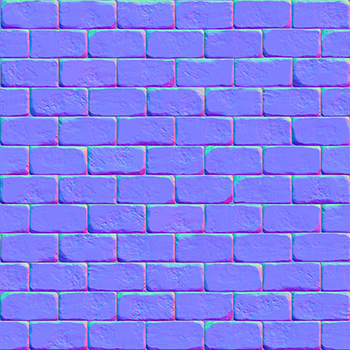
\includegraphics[width=.55\linewidth]{normalMapE}
					\end{figure}
					
					\textbf{所以,在不经过任何处理的情况下,法线贴图的法线只能对于朝向Z轴的面使用了,否则纹理的法线信息将发生错误}。因而为了解决这个问题,需要引入切线空间,将光照转换到法线贴图坐标中(\textbf{统一参照物}),然后进行应用。
					
					在一个不同的坐标空间中进行光照,这个坐标空间里,法线贴图向量总是指向这个坐标空间的正z方向;所有的光照向量都相对与这个正z方向进行变换。这样我们就能始终使用同样的法线贴图,不管朝向问题。这个坐标空间叫做\textbf{切线空间(tangent space)}。
					
				\subparagraph{切线空间}
					法线贴图中的法线向量定义在切线空间中,在切线空间中,\textbf{法线永远指着正z方向}。\underline{切线空间}是\textit{位于三角形表面之上的空间:法线相对于单个三角形的本地参考框架}。
					
					它就像法线贴图向量的\textit{本地空间};它们都被定义为指向正z方向,无论最终变换到什么方向。\textit{使用一个特定的矩阵}就能将\textit{本地/切线空间中的法线向量}\underline{转成}\textbf{世界或视图空间}下,使它们转向到最终的贴图表面的方向。
					
					法线贴图被定义在切线空间中,所以一种解决问题的方式是\textit{计算出一种矩阵,把法线从切线空间变换到一个不同的空间,这样它们就能和表面法线方向对齐了:法线向量都会指向正y方向。}\textbf{切线空间的一大好处是我们可以为任何类型的表面计算出一个这样的矩阵,由此我们可以把切线空间的z方向和表面的法线方向对齐}。
					
					\textit{这种矩阵叫做TBN矩阵这三个字母分别代表tangent、bitangent和normal向量}。这是建构这个矩阵所需的向量。要建构这样一个把切线空间转变为不同空间的变异矩阵,我们需要三个相互垂直的向量,它们沿一个表面的法线贴图对齐于:上、右、前。
					
					已知上向量是表面的法线向量(\textit{Normal})。右和前向量是切线(\textit{Tagent})和副切线(\textit{Bitangent})向量。如下所示一个表面的三个向量:
					\begin{figure}[H]
						\centering
						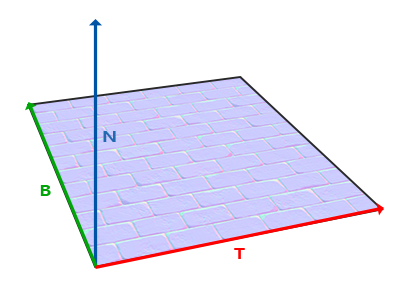
\includegraphics[width=.55\linewidth]{TBN}
						\caption{TBN 切线坐标系}
					\end{figure}
					
					如何推倒TBN矩阵 参考ref 链接即可。\textbf{至此,法线贴图就能转换到世界坐标或者视图坐标中,正确的参与计算了}。
				
					
			\paragraph{示例}
			
				直接使用TBN矩阵,把通过采样得到的\textbf{法线坐标左乘上TBN矩阵,转换到世界坐标空间中},这样所有法线和其他光照变量就在同一个坐标系中(MVP后的坐标系)了,所以只需要转换法线即可。
				\dirtree{%
					.1 方案一: .
					.2 在CPU 期间计算 切线向量、副切线向量.
					.2 在VS 阶段构造出 TBN 矩阵 .
					.2 在FS 阶段根据TBN矩阵 转换法线 .
				}
				
				 使用TBN矩阵的逆矩阵,这个矩阵可以\textbf{把世界坐标空间的向量转换到切线坐标空间}。因此使用这个矩阵左乘其他光照变量,把他们转换到切线空间,这样法线和其他光照变量再一次在一个坐标系中了。
				 
				 在像素着色器中\textit{不用对法线向量变换},\textbf{但要把其他相关向量转换到切线空间},它们是lightDir和viewDir。这样每个向量还是在同一个空间(切线空间)中了。
				 
				\dirtree{%
					.1 方案二:.
					.2 在CPU 期间计算 切线向量、副切线向量.
					.2 在VS 阶段构造出 TBN \textbf{逆矩阵}, 转换光照(方向)、视角(方向)、位置.
					.2 在FS 阶段根据TBN矩阵 .
				}			
				
				
				\subparagraph{比较}
					第二种方法看似要做的更多,它还需要在像素着色器中进行更多的乘法操作,所以为何还用第二种方法呢?
					
					将向量从世界空间转换到切线空间有个额外好处,我们可以把所有相关向量在顶点着色器中转换到切线空间,不用在像素着色器中做这件事。这是可行的,因为lightPos和viewPos不是每个fragment运行都要改变,对于fs\_in.FragPos,我们也可以在顶点着色器计算它的切线空间位置。基本上,不需要把任何向量在像素着色器中进行变换,而第一种方法中就是必须的,因为采样出来的法线向量对于每个像素着色器都不一样。
					
					所以现在不是把TBN矩阵的逆矩阵发送给像素着色器,而是将切线空间的光源位置,观察位置以及顶点位置发送给像素着色器。这样我们就不用在像素着色器里进行矩阵乘法了。这是一个极佳的优化,因为顶点着色器通常比像素着色器运行的少。这也是为什么这种方法是一种更好的实现方式的原因。
					
					
			
		\subsection{视差贴图}
			视差贴图Parallax Mapping,又称为 Offset Mapping,以及virtual displacement mapping),于2001年由Kaneko引入,由Welsh进行了改进和推广。视差贴图是一种改进的Bump Mapping技术,相较于普通的凹凸贴图,视差贴图技术得到凹凸效果得会更具真实感(如石墙的纹理将有更明显的深度)。视差贴图是通过替换渲染多边形上的顶点处的纹理坐标来实现的,而这个替换依赖于一个关于切线空间中的视角(相对于表面法线的角度)和在该点上的高度图的方程。
			
		\subsection{浮雕贴图}
			浮雕贴图(Relief Mapping),有人把它誉为\textbf{凹凸贴图的极致}。我们知道,Parallax Mapping是针对Normal Mapping的改进,利用HeightMap进行了近似的Texture Offset。而Relief Mapping是精确的Texture Offset,所以在表现力上比较完美。
	
	\section{纹理格式}
	
	
	
	\section{参考}
		参考于:\url{https://zhuanlan.zhihu.com/p/27551369}
		
		法线贴图:\url{https://www.zhihu.com/people/zheng-hua-31-46/following}
		
		
				
\chapter{光照、阴影}
	\section{学习教程}
		现代计算机图形学:笔记链接\url{https://www.notion.so/GAMES101-b0e27c856cde429b8672671a54c34817}
		
			\url{https://zhuanlan.zhihu.com/p/49474631}
			
		课件:Lecture8
		
		\textbf{Shading}:The process of \textbf{applying a material} to an object.
		
	\section{理论整理}
			\dirtree{%
				.1 虚拟环境真实感构成要素 .
				.2 光照模型 .
				.3 灯光 .
				.3 阴影 .
				.2 材质 .
				.3 明暗模型 .
				.3 纹理 .
				.3 透明.
				.3 贴图.
				}
		
	\section{光照模型}
		当光照射到物体表面时,物体对光会发生反射、透射、吸收、衍射、折射、和干涉,其中被物体吸收的部分转化为热,反射、透射的光进入人的视觉系统,使我们能看见物体。为模拟这一现象,需要建立一些数学模型来替代复杂的物理模型,这些模型就称为\textbf{明暗效应模型}或者\textbf{光照模型}。
	
		\subsection{局部光照模型}
			在真实感图形学中,\textbf{仅处理光源直接照射物体表面的光照模型}被称为\underline{局部光照明模型}。
			
			局部光照模型是一种比较简单的光照模型它是与光栅化渲染算法相适应的,光栅化算法一次只考虑一个像素的光照强度,因此局部光照模型不能计算某像素受其他像素影响的光照强度部分。也就是说,局部光照模型只对物体进行直接光照的计算,而不考虑其他的间接影响。
			
			其中典型的几个光照模型如下所示:
			
			\dirtree{%%
				.1 局部光照模型.
				.2 Lambert 漫反射模型 .
				.2 Gourand 光照模型 .
				.2 \textbf{Phong 光照模型} .
				.2 Blinn-Phong 模型 .
				.2 Cook-Torrance 模型 .
			}
			
			\paragraph{Blinn-Phong:Diffuse}
				漫反射指的是粗糙的物体表面各个方向等强度地反射光,即等同的各个方向散射的现象。继而:
				\textbf{漫反射会将到达表面的光均匀发散到所有的方向,并且各个方向观看到的颜色值相同},效果如下所示:
				\begin{figure}[H]
					\centering
					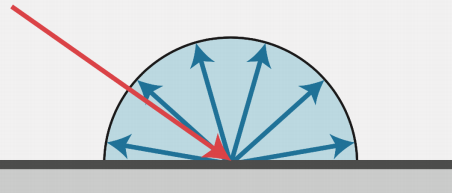
\includegraphics[width=.5\linewidth]{DiffuseModel}
					\caption{漫反射模型}
				\end{figure}
				
				其次需要明确的是,到达表面的光的能量I 能够到达多少\textbf{量},这个就需要考虑到光与表面的角度。
				\begin{figure}[H]
					\centering
					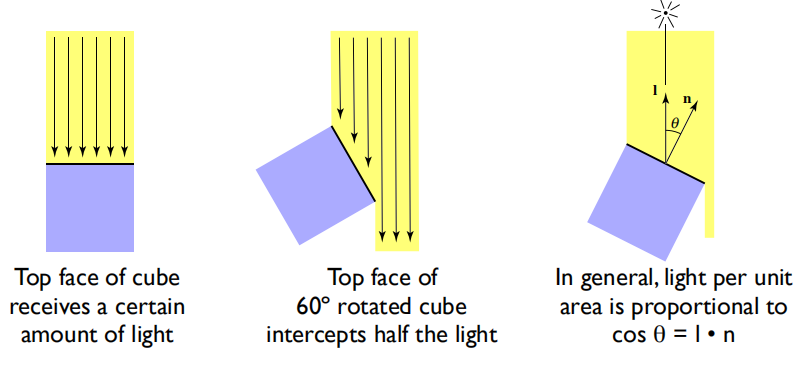
\includegraphics[width=\linewidth]{DiffuseModel02}
					\caption{漫反射:光的角度对光能接收量的影响}
				\end{figure}				
				
				最后,单位能量的光源I,在传播一定距离R 后,到达表面的能量\textbf{强度}的表示满足反比关系,如下所示。
				
				\begin{figure}[H]
					\centering
					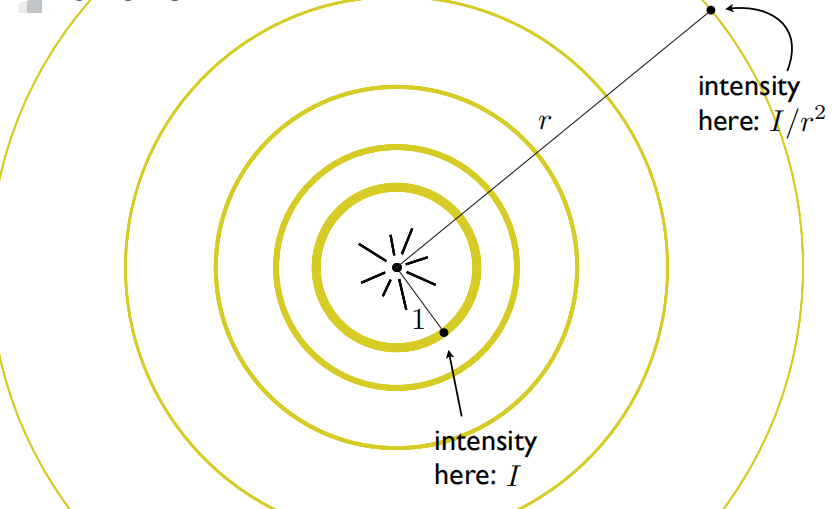
\includegraphics[width=.9\linewidth]{DiffuseModel03}
					\caption{漫反射:距离对能量的影响}
				\end{figure}				
								
				最终光照的漫反射模型如下:
				
				\begin{figure}[H]
					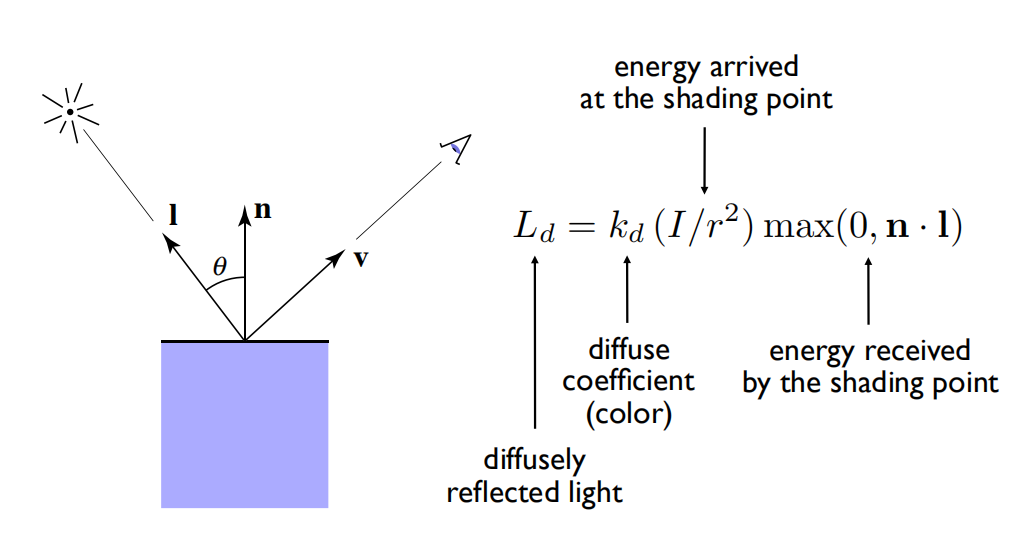
\includegraphics[width=\linewidth]{LightBasic}
					\caption{漫反射基本公式}
				\end{figure}
				
				其中的kd 表示光照漫反射系数,取值范围为(0,1),用于描述漫反射物体与环境光交互\textbf{反射的光强},既值越大,反射的量能越高,效果如下所示。
				\begin{figure}[H]
					\centering
					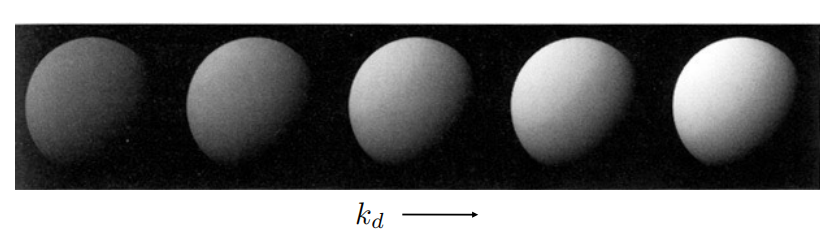
\includegraphics[width=.9\linewidth]{DiffuseModel04}
					\caption{漫反射:漫反射系数}
				\end{figure}				
			
			\paragraph{Blinn-Phong: Specular}
				模型如下:
				
				\begin{figure}[H]
					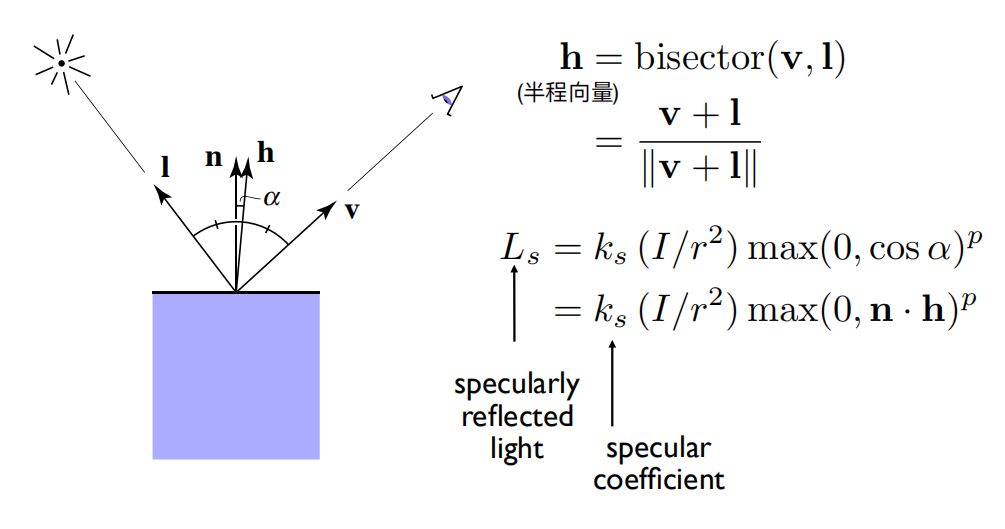
\includegraphics[width=\linewidth]{LightBasic-02}
					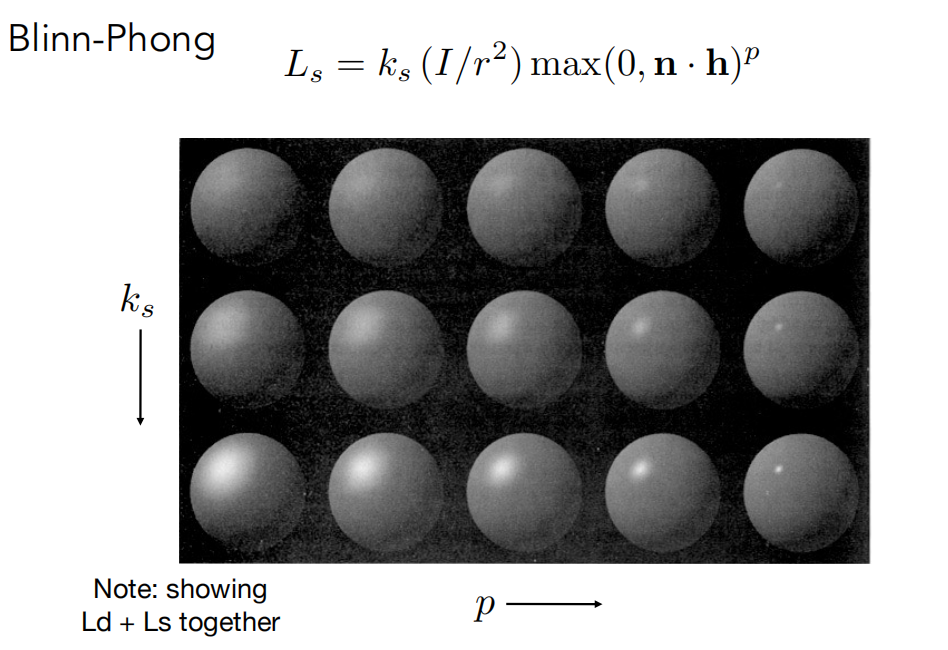
\includegraphics[width=\linewidth]{LightBasic-03}
					\caption{高光基本公式}
				\end{figure}				
			
			\paragraph{Blinn-Phong: Ambient}
				模型如下:
				
				\begin{figure}[H]
					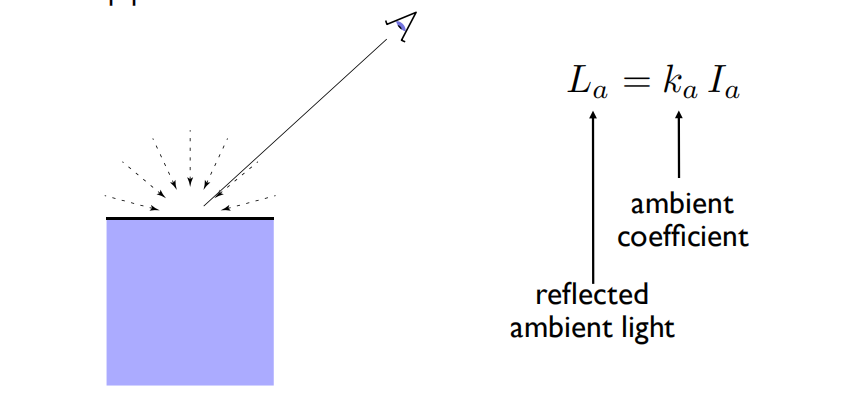
\includegraphics[width=\linewidth]{LightBasic-04}
					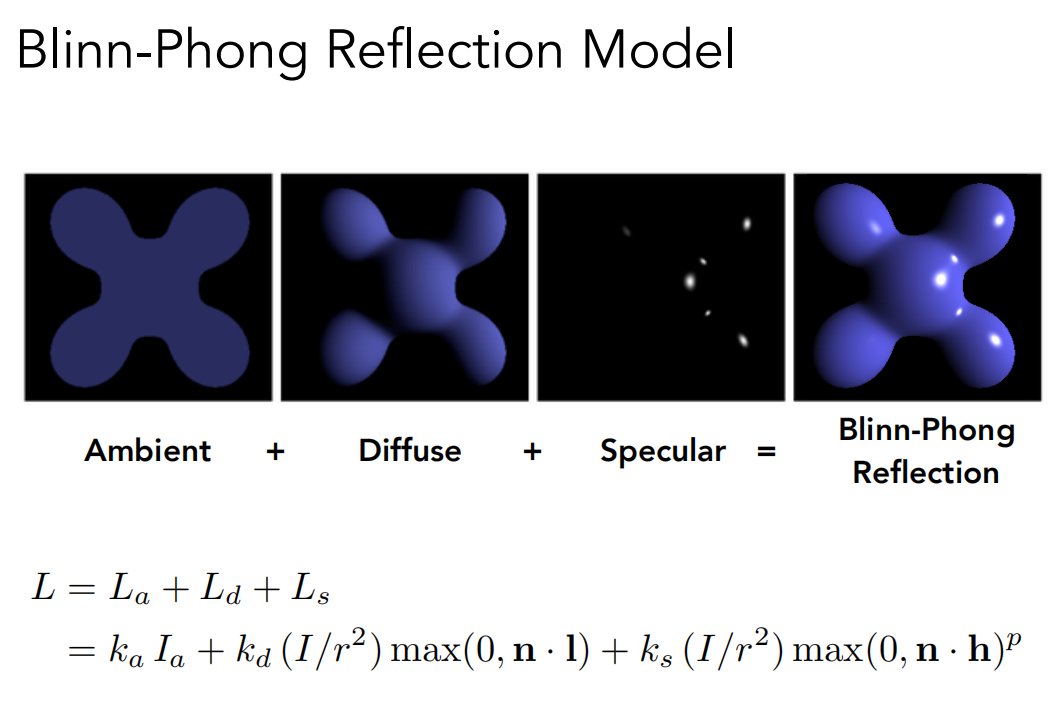
\includegraphics[width=\linewidth]{LightBasic-05}
					\caption{环境光基本公式}
				\end{figure}			
			
			
			\paragraph{Shader 应用}
				如何在 像素着色器中应用 光照渲染。
				
				首先需要一个光线方向,其次需要像素的法线方向,最后需要的是光照强度等一些列常数参数。
				
			
				而\textbf{像素的基础颜色}从哪里来,这就需要纹理贴图相关的知识,这部分参考纹理一章。
				
				\begin{lstlisting}[frame=L]
	uniform sampler2D myTexture; // program parameter
	uniform vec3 lightDir; // program parameter 
	varying vec2 uv; // per fragment value (interp. by rasterizer) 
	varying vec3 norm; // per fragment value (interp. by rasterizer)
	void diffuseShader() 
	{ 
		vec3 kd; 
		kd = texture2d(myTexture, uv); // material color from texture
		kd *= clamp(dot(–lightDir, norm), 0.0, 1.0); // Lambertian shading model
		gl_FragColor = vec4(kd, 1.0); // output fragment color
	}								
				\end{lstlisting}
				
		\subsection{全局光照模型}
			全局光照模型是\textbf{基于光学物理原理的},光照强度的计算依赖于光能在现实世界中的传播情况,考虑光线与整个场景中各物体表面及物体表面间的相互影响,包括多次反射 、透射 、散射等。因此,与局部光照模型相比,全局光照模型需要相当大的计算量 ,但同时也能取得非常逼真的真实效果 。
		
			\dirtree{%
				.1 全局光照模型.
				.2 \textbf{光线跟踪} .
				.3 路径追踪()Path Tracing).
				.3 递归光线追踪()whitted-type).
				.3 分布式光线追踪(Distribution).
				.3 双向路径追踪(Bidirtional Path) .
				.3 Metropolis .
				.3 光子映射(Photon Mapping) .
				.3 基于点的全局光照 .
				.2 辐射度算法 .
				.2 光子映射 .
			}			
			
			\paragraph{光线追踪}
			
			\paragraph{whitted光线追踪}
			
			\paragraph{分布式光线跟踪}
			
			\paragraph{辐射度}
			
			\paragraph{光子映射}
			
	\section{阴影原理}
	
		其中遮挡物(occluders)是将阴影投射到接收器(receivers)上的对象。精确光源(Punctual light sources),即没有面积的光源,只会产生完全阴影的区域,有时也称为硬阴影(hard shadows)。如果使用区域光(area light)或体积光(volume light),则会产生柔和的阴影。这样,每个阴影都可以具有称为“本影”(umbra)的完全阴影区域和称为“半影”(penumbra)的部分阴影区域。拥有模糊边缘的阴影,是软阴影。如下图所示:
	
			\begin{figure}[H]
				\centering
				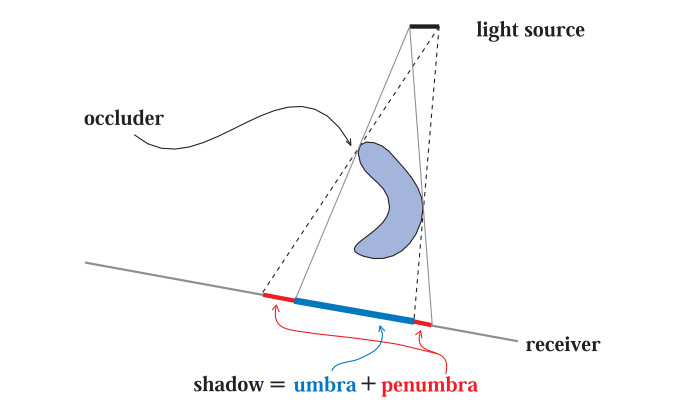
\includegraphics[width=\linewidth]{Shadow01}
				\caption{阴影组成示例:光源、遮挡物、接受体,阴影,硬阴影,软阴影}
			\end{figure}
				
			\begin{figure}[H]
				\centering
				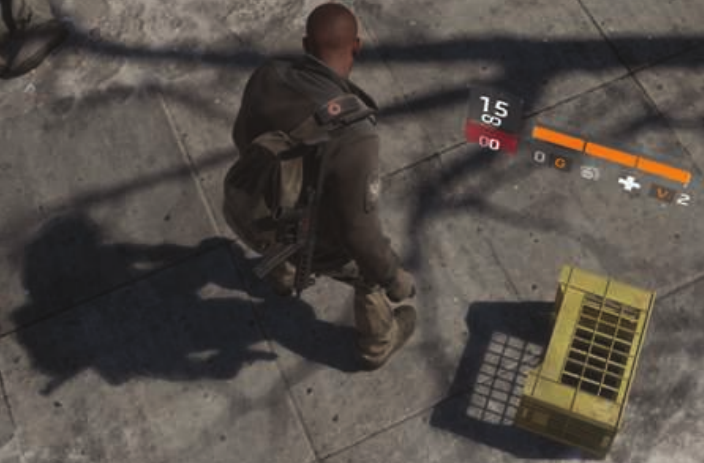
\includegraphics[width=\linewidth]{Shadow02}
				\caption{硬阴影和软阴影的混合}
			\end{figure}			
			由于遮挡物靠近接收器,因此板条箱的阴影很锐利。该人的阴影在接触点处很锐利,随着与封堵器距离的增加而变柔和。遥远的树枝给人柔和的阴影。
			
		\subsection{平面阴影}
			\paragraph{投影阴影}
				ref:\url{https://learnopengl-cn.github.io/05%20Advanced%20Lighting/03%20Shadows/01%20Shadow%20Mapping/}
			
				\textbf{阴影映射}(Shadow Mapping):\textit{以光的位置为视角进行渲染,能看到的东西都将被点亮,看不见的一定是在阴影之中了}。假设有一个地板,在光源和它之间有一个大盒子。由于光源处向光线方向看去,可以看到这个盒子,但看不到地板的一部分,这部分就应该在阴影中了
				
				\begin{figure}[H]
					\centering
					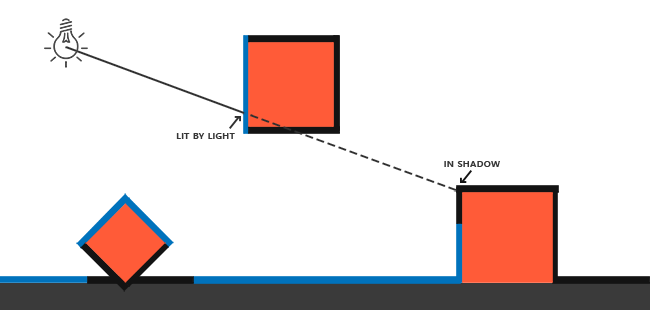
\includegraphics[width=\linewidth]{shadow_mapping_theory}
					\caption{投射原理}
				\end{figure}
			
				在深度缓冲里的一个值是摄像机视角下,对应于一个片段的一个0到1之间的深度值。如果我们\textbf{从光源的透视图来渲染场景},并把深度值的结果储存到纹理中会怎样?通过这种方式,我们就能对光源的透视图所见的最近的深度值进行采样。最终,深度值就会显示从光源的透视图下见到的第一个片段了。我们管储存在纹理中的所有这些深度值,叫做深度贴图(depth map)或\textbf{阴影贴图}。
				
				然后最后利用像素的深度值进行判断当前像素是否有高光(没有处于阴影中),当处于阴影时,将其高光计算不参与光照明暗处理模型中即可,如
				\begin{lstlisting}
// 此部分为像素着手器核心代码。				
// 当处于阴影时,shadow 为1.0, 没有处于为0.				
vec3 lighting = (ambient + (1.0 - shadow) * (diffuse + specular)) * color; 				
				\end{lstlisting}
			
				在此方案中,三维对象会进行\textit{第二次渲染}以创建阴影。首先一次需要创建深度缓存,第二次利用深度缓存(Z-buffering) 进行渲染。
				
		
			\paragraph{以Light为出发点的矩阵变换}
				MVP矩阵变换,其中Model 继承,V(view) 可以通过glm::lookat 获取,P(projection) 可以通过glm::ortho() 获取。
					
				那么对于模型 M 的变换矩阵就是 VP. 
		
			\paragraph{Z-buffering 获取}
				深度贴图是从光的透视图里渲染的深度纹理,所以需要将场景的\textit{渲染结果储存到一个纹理}中,而这需要\textbf{帧缓冲}。
					
				具体参考OpenGL4.5 OpenGL基础/帧缓冲一章。
			
			\paragraph{软阴影}
			
			
		
		\subsection{曲面上的阴影}
		
		
		\subsection{阴影体}
		
		
		\subsection{阴影贴图}
		
		
		\subsection{百分比渐近滤波软阴影}
		
		
		\subsection{滤波阴影贴图}
		
		
		\subsection{体积阴影}
		
		
		\subsection{不规则 Z缓冲区阴影}
		
	
	
	
	
	
	
	

	
	\section{环境光遮蔽-AO}	
		参考链接:\url{https://zhuanlan.zhihu.com/p/43105945}
	
		\subsection{全局环境}
			Ambient Environments是一种技术,旨在让我们\textbf{摆脱场景中的大量补光灯}。Ambient Environments有两个组件。
			\begin{itemize}
				\item “Ambient Environment Lights”提供照明
				\item “Ambient Occlusion”提供阴影和重要的方向信息。
			\end{itemize}
			
			与\underline{反射遮挡}类似,Ambient Environments也使用\textit{在渲染时访问的预渲染遮挡贴图来为我们的场景提供逼真的阴影}。我们可以方便地为周围环境和反射环境使用相同的环境贴图。
			
			Ambient Environments代表围绕物体的漫反射填充光,\textit{它并不代表直接光源,而是模拟间接反射形成的环境光}。
		
		
		\subsection{环境光}
			环境光(Ambient environment lights)只是一种改进的环境反射。
		
			一个环境光源(ambient light source)表示全方位,固定强度和固定颜色的光源,其均等地影响场景中的所有对象。 渲染时,场景中的所有对象都会以指定的强度和颜色变亮。 这种类型的光源主要用于为场景提供其中不同对象的基本视图。 这是最简单的照明类型,可以模拟光线如何分散或反射多次,从而产生均匀的效果。
			
			\underline{环境光}可以与\underline{环境遮挡}相结合,\textbf{以表示场景中每个点的曝光方式,从而影响其可以反射的环境光量}。 这会在整个场景中产生漫反射,无方向性的照明,没有明显的阴影,但是封闭和遮蔽的区域变暗。 结果通常在视觉上与阴天相似。
			
			\textbf{特点:}使用环境光的一个显着优点是渲染成本低廉,因此特别适用于可能需要最小化场景中灯光数量的移动应用。
			
		\subsection{环境光遮蔽}
			在计算机图形学中全局光照的效果直接影响画面的真实性。使用传统的基于物理的关照算法(例如光线跟踪算法 )可以达到很好的效果但是技术计算复杂 ,难以实时,其计算复杂难以做到实时应用 。
			
			环境遮挡是创建逼真的周围环境的关键因素。 它\textbf{提供了}我们期望\textit{从全局照明和其他更复杂的间接照明技术中获得的柔和阴影}。 \textbf{未完全暴露于环境的表面上的光照需要适当地衰减,以使它们不能获得周围环境光的全部贡献}。 这是使用Ambient Environments技术的主要吸引力之一。
			
			
			\textbf{作用}:通过描绘物体之间由于遮挡而产生的阴影, 能够更好地捕捉到场景中的细节,可以解决漏光,阴影漂浮等问题,改善场景中角落、锯齿、裂缝等细小物体阴影不清晰等问题,增强场景的深度和立体感。
			
			
			\paragraph{思路}
				为了获得这种效果,有必要使用\underline{环境遮挡渲染} (Ambient Occlusion Render) 或\underline{“烘焙”环境遮挡贴图} (“baked” ambi- ent occlusion maps)\textbf{来表示外部光的衰减}。
				
				通过以下过程实现环境遮挡:对于每个表面点,光线在\underline{表面法线}(surface normal)周围的半球中投射。 \textbf{最终的遮挡量}\underline{取决于}\textit{击中场景中其他表面或物体的射线的数量}。
			
				更清晰一点描述:首先用半球罩住,然后\textbf{从半球发射无数条射线},如果直接可以反射回半球的我们就给它白色,如果因为遮挡反弹两次才回到半球我们就给它一个比较暗的颜色,反弹次数越多,得到的像素就越暗,如果没有返回到光源半球的光线,我们就给它一个黑色。
				
				这是一种计算方式,当然还要其他的计算方式,光源可以不是半球。基本的思路差不多是这样。
		
			    
			\paragraph{使用注意事项}
				由于在所有的漫反射中,\textbf{贡献度最大的来自表面法线的大致方向},因此对结果进行加权计算,以有利于向该方向投射的样本。 如果有一个直接平行于表面的物体,它将比同一个物体放置在侧面时拥有更多的遮挡。
				
				应从Ambient Occlusion渲染中\textbf{排除透明或玻璃材质}。 
				
				
			\paragraph{理论分类}
				\begin{itemize}
					\item \textbf{SSAO}-Screen space ambient occlusion
					\item SSDO-Screen space directional occlusion
					\item HDAO-High Definition Ambient Occlusion
					\item HBAO+-Horizon Based Ambient Occlusion+
					\item AAO-Alchemy Ambient Occlusion
					\item ABAO-Angle Based Ambient Occlusion
					\item PBAO
					\item VXAO-Voxel Accelerated Ambient Occlusion
				\end{itemize}
		
		\subsection{SSAO 原理分析与实现}
			屏幕空间环境光遮蔽(Screen-Space Ambient Occlusion, SSAO)。
			
			SSAO背后的原理很简单:对于铺屏四边形(Screen-filled Quad)上的每一个片段,\textit{都会根据周边深度值}计算一个\textbf{遮蔽因子(Occlusion Factor)}。这个遮蔽因子之后\textit{会被用来减少或者抵消片段的环境光照分量}。\textbf{遮蔽因子}是\textit{通过采集片段\underline{周围球型核心(Kernel)}的多个深度样本,并和当前片段深度值对比而得到的}。\textbf{高于片段深度值样本的个数就是想要的遮蔽因子}。
			
			由于球型核心会造成平面灰化,因而现在都是用的是\textbf{半球面(沿着表面法向量的半球体采样核心)}进行求遮挡因子。
			\begin{figure}[H]
				\centering
				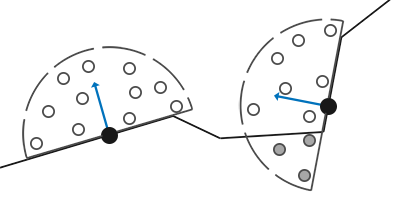
\includegraphics[width=.78\linewidth]{ssao_hemisphere}
				\caption{法线半球体 采样示例}
			\end{figure}
			
			通过在法向半球体(Normal-oriented Hemisphere)周围采样,\textbf{将不会考虑到片段底部的几何体.它消除了环境光遮蔽灰蒙蒙的感觉},从而产生更真实的结果。
			
			SSAO是一种屏幕空间技巧,是对屏幕(2D四边形)上\textbf{每一个片段(像素)}计算这一效果;也就是说我们没有场景中几何体的信息。
			能做的只是渲染几何体数据到屏幕空间纹理中的像素,之后再会将此数据发送到SSAO着色器中处理。因而需要Fram-Buffer 将需要的信息存储下来。
			
			\begin{figure}[H]
				\centering
				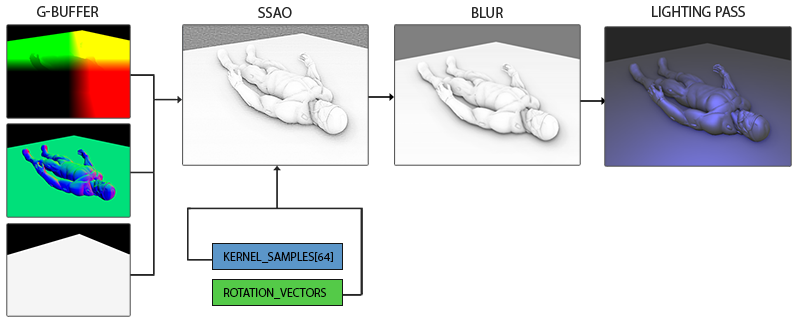
\includegraphics[width=\linewidth]{SSAO}
				\caption{流程示例}
			\end{figure}
			
			
			\paragraph{具体步骤}
				
				
			
			\paragraph{示例}
				
			
			
			
			
	\section{环境法线(Bent Normal)}
		ref:\url{https://blog.csdn.net/BugRunner/article/details/7272902}
	
		几何模型的表面法向量是必需的一个信息元素, Bent Normal是\textbf{对原始的Normal做修改之后的新向量},它指向了当前像素一个不被其它物体(或几何体元)遮挡的平均方向,也即\textbf{光线传入的主要方向}。
		
		其公式如下所示
		$$
		N_{\mathbf{b}}(\mathbf{x}) = \dfrac{1}{\pi} \int_{\Omega} V(x,\omega)\omega d\omega
		$$
		
		其中$V(x,\omega)$即为当前点$x$在$\omega$方向上的可见性,也即是否被遮挡。使用\textbf{蒙特卡罗积分}将其离散化即可得到一个\textit{有限采样下}可行的Bent Normal计算公式。
		
		\begin{figure}[H]
			\centering
			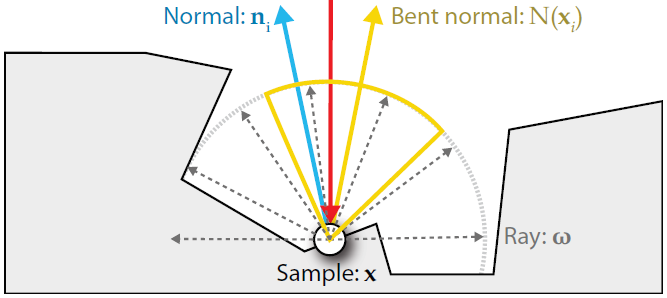
\includegraphics[width=.75\linewidth]{BentNormal}
			\caption{Bent Normal的采样示意图}
		\end{figure}
		
		从图中可以看出,\textbf{Bent Normal(黄色)}与\textbf{原始Normal(蓝色)}相比,\textit{其在考虑周围几何体元分布的情况下向右侧做了修整}。
		
		\paragraph{用法}Bent Normal一般来说可以有两种用途
		
			\begin{itemize}
				\item 用来改变原始的Normal,并记录光线的主要通过方向,这样在做环境贴图的采样时可以从更优化的方向来计算采样的光线。
				\item 用来代替原始的Normal做正常的Shading,这样可以在尽管只有Normal的情况下一定程度上得到类似于Ambient Occlusion的Soft Shadow效果。
			\end{itemize}
			
		
		\paragraph{计算方式}
			Bent Normal的计算方式一般来说也有两种方法
			
			\begin{itemize}
				\item \textbf{传统的离线采样方法},这里的操作就跟传统offline的Ambient Occlusion计算方法一样,在场景的表面上的每个点处做采样,并计算【式一】的蒙特卡罗积分即可统计得到考虑场景遮挡情况下的Bent Normal。
				\item \textbf{基于Screen Space的方法},其优点就是快、缺点就是不太精确。为了在游戏中得到实时的AO计算,众多基于屏幕空间的SSAO算法被提出来,而AO 的计算又与Bent Normal的计算是相关的,因而就可以\textit{使用通常的SSAO post pass来将Bent Normal无过多额外代价的快速计算出来(但是会多出一个Normal  buffer的采样,或以合适的方法避免之)}。具体的操作也跟AO的计算类似,只不过在每个屏幕采样点处将相应的AO 值转化为对Normal 的偏移即可。
			\end{itemize}
		
		
	\section{UE4 实践}
		
		
		
			

\chapter{视觉:抗锯齿、透明}
	\section{抗锯齿与常见抗锯齿类型}
		抗锯齿(英语:Anti-Aliasing,简称AA),也译为边缘柔化、消除混叠、抗图像折叠有损,反走样等。它是一种消除显示器输出的画面中图物边缘出现凹凸锯齿的技术,那些凹凸的锯齿通常因为高分辨率的信号以低分辨率表示或无法准确运算出3D图形坐标定位时所导致的图形混叠(aliasing)而产生的,抗锯齿技术能有效地解决这些问题。
		
		下面将常见的几种抗锯齿类型进行总结介绍,也包括RTR3中没有讲到的,最近几年新提出的常见抗锯齿类型。
		
		\subsection{超级采样抗锯齿(SSAA)}
		
		\subsection{多重采样抗锯齿(MSAA)}
		
		\subsection{覆盖采样抗锯齿(CSAA)}
		
		\subsection{高分辨率抗锯齿(HRAA)}
		
		\subsection{可编程过滤抗锯齿(CFAA)}
		
		\subsection{形态抗锯齿(MLAA)}
		
		\subsection{快速近似抗锯齿(FXAA)}
		
		\subsection{时间性抗锯齿(TXAA)}
		
		\subsection{多帧采样抗锯齿(MFAA)}
		
	\section{透明渲染与透明排序}
		\subsection{透明渲染}
		
		\subsection{透明排序}
			\paragraph{深度缓存(Z-Buffer)}
			
			\paragraph{画家算法(Painter's Algorithm)}
			
			\paragraph{加权平均值算法(Weighted Average)}
			
			\paragraph{深度剥离算法(Depth Peeling)}

	\section{伽马矫正}
	
	\section{参考文献}
			参考于:\url{https://zhuanlan.zhihu.com/p/27234482}
	


\chapter{参考学习路线}					
	
	\section{OS 基础}
		《Programming Windows 5th》只需要看前面几章,理解 Win32 消息循环即可。
	
		《Multithreading Applications in Win32》,理解多线程是怎么回事;
	
	\section{GUI}
	 	WPF、MFC
	
	\section{3D 图形学}
		二选一,我推荐 handmadehero,因为有很详细的视频教程。
		
		\url{https://handmadehero.org/}
		
		\url{http://frustum.org/3d/}从最开始的 demo 开始,用 DX 全部写一遍。
	
	\section{基础篇}
		\begin{itemize}
			\item 上篇,各种概念与技术。《Fundamentals of Computer Graphics 3rd》 or 《Computer Graphics - Principles and Practice》
			\item 中篇,各种算法。《Real-Time Rendering 4th》
			\item 下篇,高阶追求。《Physically Based Rendering - From Theory To Implementation 2nd》
			\item 杂篇1,只谈数学,《3D Math Primer for Graphics and Game Development 2nd》
			\item 杂篇2,同上,《Mathematics for 3D Game Programming and Computer Graphics 3rd》
		\end{itemize}
		
	\section{API 之术(DX9/11 or OpenGL)}
		\begin{itemize}
			\item 《3D绘图程序设计》,dx9/10/ogl 实现各种3D游戏需要的效果
			\item 《More OpenGL Game Programming》,如何用 gl 实现各种中高级效果
			\item 《Introduction to 3D Game Programming with DirectX 9.0c - A Shader Approach》,龙书
			\item 《Introduction to 3D Game Programming with DirectX 11》,龙书 DX11 版
			\item 《Practical Rendering and Computation with Direct3D 11》,DX11 宝典
			\item 《OpenGL Programming Guide》,OpenGL 宝典		
			\item 《OpenGL Shading Language》,glsl 宝典			
		\end{itemize}
	
	\section{引擎设计}		
		David Eberly 的《3D Game Engine Design》,WildMagic,这有一个完整的引擎实现
		
		Jason Gregory 的《Game Engine Architecture》
		
		《Character Animation with Direct3D》,专注讲 model、animation 的。
		
	\section{各种技巧}
		ShaderX 系列
		《Real Time Collision Detection》
		《Real Time Cameras》
		《Real-Time Shadows》

	  
\end{document} 
 		    